% This is samplepaper.tex, a sample chapter demonstrating the
% LLNCS macro package for Springer Computer Science proceedings;
% Version 2.20 of 2017/10/04
%
\documentclass[runningheads]{llncs}
%
\usepackage{graphicx}
% Used for displaying a sample figure. If possible, figure files should
% be included in EPS format.
%
% If you use the hyperref package, please uncomment the following line
% to display URLs in blue roman font according to Springer's eBook style:
% \renewcommand\UrlFont{\color{blue}\rmfamily}
\usepackage[labelformat=simple]{subcaption}
% \renewcommand\thesubfigure{(\alph{subfigure})}
\renewcommand{\thesubfigure}{(\roman{subfigure})}
\usepackage{floatrow} % for caption beside the figure --- use the \floatbox and \capbeside commands provided by the floatrow package
\usepackage{amsmath,epstopdf}
\usepackage{enumerate}
\usepackage{amssymb}
\usepackage{setspace}
\usepackage[linesnumbered, ruled, vlined, noend]{algorithm2e}
% \usepackage{tabularray} %for new style table
% \UseTblrLibrary{booktabs}
% \usepackage{amsthm}
\usepackage{color}
\usepackage[]{color}
\usepackage[]{url}
\usepackage[colorlinks,linkcolor=black,urlcolor=black,citecolor=black]{hyperref}

\usepackage{cleveref}
\newenvironment{appendix-lemma}[1]{\vspace{0.1in}\noindent{\bf Lemma~#1~} \em }{\vspace{0.1in}}
\newenvironment{appendix-claim}[1]{\vspace{0.1in}\noindent{\bf Claim~#1~} \em }{\vspace{0.1in}}
\newenvironment{appendix-theo}[1]{\vspace{0.1in}\noindent{\bf Theorem~#1~} \em }{\vspace{0.1in}}
\usepackage{tikz}
\usepackage{standalone}
\usetikzlibrary{arrows}
\usetikzlibrary{decorations,fit,shapes} 
\usetikzlibrary{decorations.markings}
\usetikzlibrary{arrows.meta,positioning}
\usetikzlibrary{shapes.misc}
\tikzset{cross/.style={cross out, draw=black, minimum size=2*(#1-\pgflinewidth), inner sep=0pt, outer sep=0pt},
	%default radius will be 1pt. 
	cross/.default={1pt}}
\usetikzlibrary{arrows, decorations.pathmorphing}
%\newcommand \mydots{\hbox to 0.8em{.\hss .\hss .}}
%\newcommand \myDots{\hbox to 0.8em{....}}

\tikzstyle{vertex}=[auto=left,circle,draw=black!80,fill=none,minimum size=15pt,inner sep=0pt]

%tik picture
%\usepackage{comment}
\tikzset{
	photon/.style={decorate, decoration={snake}, draw=red}} 


% \newenvironment{appendix-lemma}[1]{\vspace{\theorempreskipamount}\noindent{\bf Lemma~#1~} \em }{\vspace{\theorempostskipamount}}
\newcommand{\etal}{\textit{et al}. }



\begin{document}
	%
	\title{Critical Relaxed Stable Matchings with Two-Sided Ties} %TODO Please add
	%\titlerunning{Abbreviated paper title}
	% If the paper title is too long for the running head, you can set
	% an abbreviated paper title here
	%
	
	\titlerunning{Critical Relaxed Stable Matchings with Two-Sided Ties} %TODO optional, please use if title is longer than one line
	
	
	\author{Meghana Nasre\inst{1} \and
		Prajakta Nimbhorkar\inst{2} \and
		Keshav Ranjan\inst{1}}
	%
	%\authorrunning{F. Author et al.}
	% First names are abbreviated in the running head.
	% If there are more than two authors, 'et al.' is used.
	%
	\authorrunning{M. Nasre et al.} %TODO mandatory. First: Use abbreviated first/middle names. Second (only in severe cases): Use first author plus 'et al.'
	\institute{IIT Madras, Chennai, India \and
		Chennai Mathematical Institute and UMI ReLaX, India}
	%
	
	%%%%%%%%%%%%%%%%%%%%%%%%%%%%%%%%%%%%%%%%%%%%%%%%%%%%%%
	\newcommand{\Poly}{\mbox{{\sf P}}}
	\newcommand{\HR}{\mbox{{\sf HR}}}
	\newcommand{\HRTLQ}{\mbox{{\sf HR2LQ}}}
	\newcommand{\prefa}{\mbox{{\sf Pref($a$)}}}
	\newcommand{\prefap}{\mbox{{\sf Pref($a_1$)}}}
	\newcommand{\prefal}{\mbox{{\sf List($a$)}}}
	\newcommand{\preflqa}{\mbox{{\sf PrefC($a$)}}}
	\newcommand{\prefb}{\mbox{{\sf Pref($b$)}}}
	\newcommand{\prefr}{\mbox{{\sf Pref($r$)}}}
	\newcommand{\prefsa}{\mbox{{\sf PrefS($a$)}}}
	\newcommand{\prefslqa}{\mbox{{\sf PrefSC($a$)}}}
	\newcommand{\prefu}{\mbox{{\sf Pref($u$)}}}
	\newcommand{\prefv}{\mbox{{\sf Pref($v$)}}}
	\newcommand{\HRLQ}{\mbox{{\sf HRLQ}}}
	\newcommand{\SMLQ}{\mbox{{\sf SM-1C}}}
	\newcommand{\RSM}{\mbox{{\sf RSM}}}
	\newcommand{\RWSM}{\mbox{{\sf RSM}}}
	\newcommand{\CRWSM}{\mbox{{\sf CRITICAL-RSM}}}
	\newcommand{\MCRWSM}{\mbox{{\sf MAX-CRITICAL-RSM}}}
	\newcommand{\POP}{\mbox{{\textsc{AlgoPop}}}}
	\newcommand{\MMLQ}{\mbox{{\sf MM2LQ}}}
	\newcommand{\SMTTLQ}{\mbox{{\sf SMTIC}}}
	\newcommand{\SMTI}{\mbox{{\sf SMTI}}}
	\newcommand{\HRTTLQ}{\mbox{{\sf HR-2T-2LQ}}}
	\newcommand{\LQ}{\mbox{{\sf LQ}}}
	
	\newcommand{\CL}{\mbox{{\sf CL}}}
	\newcommand{\Df}[1]{\mbox{{\sf $def(#1)$}}}
	\newcommand{\Dfa}[1]{\mbox{{\sf $def_{\mathcal{A}}(#1)$}}}
	\newcommand{\Dfb}[1]{\mbox{{\sf $def_{\mathcal{B}}(#1)$}}}
	\newcommand{\Dfh}[1]{\mbox{{\sf $def_{\mathcal{H}}(#1)$}}}
	\newcommand{\Dfr}[1]{\mbox{{\sf $def_{\mathcal{R}}(#1)$}}}
	\newcommand{\MAXEFM}{\mbox{{\sf MAXEFM}}}
	\newcommand{\MAXSMTI}{\mbox{{\sf MAX SMTI}}}
	\newcommand{\CLIQUE}{\mbox{{\sf CLIQUE}}}
	\newcommand{\minBP}{\mbox{{\sf MinBP}}}
	\newcommand{\minBR}{\mbox{{\sf MinBR}}}
	\newcommand{\ESDA}{\mbox{{\sf ESDA}}}
	\newcommand{\MSDA}{\mbox{{\sf MSDA}}}
	\newcommand{\CSM}{\mbox{{\sf CSM}}}
	\newcommand{\EFHRLQ}{\mbox{{\sf{EF}\text{-}\sf{HR}\text{-}\sf{LQ}}}}
	\newcommand{\HH}{\mathcal{H}}
	\newcommand{\RR}{\mathcal{R}}
	\renewcommand{\AA}{\mathcal{A}}
	\newcommand{\BB}{\mathcal{B}}
	\newcommand{\CC}{\mathcal{C}}
	\newcommand{\RRLQ}{\mathcal{R}_{lq}}
	\newcommand{\HHLQ}{\mathcal{H}_{lq}}
	\newcommand{\AALQ}{\mathcal{A}_{lq}}
	\newcommand{\AANLQ}{\mathcal{A}_{nlq}}
	\newcommand{\BBLQ}{\mathcal{B}_{lq}}
	\newcommand{\BBNLQ}{\mathcal{B}_{nlq}}
	\newcommand{\lst}{list}
	\newcommand{\lqlst}{lqlist}
	\newcommand{\clst}{clonedlist}
	\newcommand{\D}{\mathcal{D}}
	\newcommand{\EE}{\mathcal{E}}
	\newcommand{\clr}{\textcolor{blue}}
	\newcommand{\rvrO}{\textcolor{blue}}
	\newcommand{\rvrT}{\textcolor{orange}}
	\newcommand{\rvrTh}{\textcolor{cyan}}
	\newcommand{\clrR}{\textcolor{red}}
	\newcommand{\comment}{\textcolor{red}}
	\renewcommand{\S}{{s}}
	\newcommand{\T}{{t}}
	
	
	\newcommand{\cor}{{\bf corr}}
	\newcommand{\tG}{\tilde{G}}
	%\newcommand{\tM}{\tilde{M}}
	\newcommand{\tHH}{\tilde{\mathcal{H}}}
	\newcommand{\tL}{\mathcal{L'}}
	\newcommand{\tLR}{\tilde{\mathcal{L}_r}}
	\newcommand{\tLH}{\tilde{\mathcal{L}_h}}
	\newcommand{\dL}{\mathcal{D}'}
	\newcommand{\dLA}{\mathcal{D}_A'}
	\newcommand{\dLB}{\mathcal{D}_B'}
	\newcommand{\tLA}{\mathcal{L}'_A}
	\newcommand{\tLB}{\mathcal{L}'_B}
	\newcommand{\tE}{\tilde{{E}}}
	
	\newtheorem{cl}{Claim}
	\newtheorem{obs}[theorem]{Observation}
	
	\maketitle              % typeset the header of the contribution
	%
	\begin{abstract}
		We consider the stable marriage problem in the presence of ties in preferences and critical vertices. The input to our problem is a bipartite graph $G = (\AA \cup \BB, E)$ where $\AA$ and $\BB$ denote sets of vertices which need to be matched. Each vertex has a preference ordering over its neighbours  possibly containing ties. In addition, a subset of  vertices in $\AA \cup \BB$ are marked as critical and the goal is to output a matching that matches as many critical vertices as possible. Such matchings are called critical matchings in the literature and in our setting, we seek to compute a matching that is critical as well as optimal with respect to the preferences of the vertices. 
		
		Stability, which is a well-accepted notion of optimality in the presence of two-sided preferences, is generalized to weak-stability in the presence of ties. It is well known that in the presence of critical vertices, a matching that is critical as well as weakly stable may not exist. 
		Popularity is another well-investigated notion of optimality for the two-sided preference list setting, however,  in the presence of ties (even with no critical vertices), a popular matching need not exist. 
		We, therefore, consider the notion of relaxed stability which was introduced  and studied by  Krishnaa~et.~al. (SAGT 2020). We show that a critical matching which is relaxed stable always exists in our setting although computing a maximum-sized relaxed stable matching turns out to be NP-hard. Our main contribution is a 3/2 approximation to the maximum-sized critical relaxed stable matching for the stable marriage problem with two-sided ties and critical vertices.
		
		
		\keywords{Stable Matching \and Two-Sided Ties \and Critical \and Relaxed Stable \and Approximation Algorithm.}
	\end{abstract}
	%
	%
	%
	\section{Introduction}\label{sec:intro}
We study the stable marriage problem in the presence of {\em ties} in preferences and {\em critical vertices}. 
 Formally, the input to our problem is a bipartite graph $G=(\AA\cup\BB,E)$, where $\AA$ and $\BB$ are two sets of vertices and $E$ denotes the set of all the acceptable vertex-pairs. %Every vertex $u\in \AA\cup\BB$ has a preference ordering on its neighbours, called the {\em preference list} of $u$, denoted as $\prefu$. 
 Each vertex $u \in \AA \cup \BB$ ranks a subset of vertices in the other partition (its neighbours in $G$)  in order of its preference possibly involving ties -- this ordering is denoted as $\prefu$. 
 For a vertex $u$ let $v_1$ and $v_2$ be its neighbours in $G$. The vertex $u$ strictly prefers $v_1$ over $v_2$  (denoted as $v_1 \succ_u v_2$) if the rank of the edge $(u, v_1)$ is smaller than the rank of the edge $(u, v_2)$.  The vertex $u$ is tied
 between $v_1$ and $v_2$ (denoted as $v_1 =_u v_2$) if the ranks on the edges $(u, v_1)$ and $(u, v_2)$ are the same. We use  $v_1\succeq_u v_2$ to denote that the rank of $v_1$ is at least as good as the rank of $v_2$ in $\prefu$.
In addition, the input consists of a set $\CC\subseteq (\AA\cup\BB)$ of \emph{critical vertices}. %Our goal is to compute a matching in $G$ that matches maximum number of critical vertices. 
Critical vertices are a generalization of lower-quota vertices that {\em must} be matched in any assignment. In our setting, critical vertices can be left unassigned, however, we wish to minimize the number of critical vertices left unassigned.
%\clr{In literature, the stable marriage problem with ties and incomplete lists is denoted by \SMTI. We denote our setting -- the stable marriage problem with two-sided ties and two-sided critical vertices by \SMTTLQ. Note that we allow the preference lists to be incomplete in our setting.}

A \emph{matching} $M\subseteq E$ in $G$ is a set of edges that do not share an end-point. For each vertex $u\in\AA\cup\BB$, we denote by $M(u)$, the neighbour of $u$ that is assigned to $u$ in $M$. %In the matching $M$, a vertex $u\in\AA\cup\BB$ is called \emph{matched} if $|M(u)| = 1$ and \emph{unmatched} if $|M(u)| =0$. %A critical vertex $u$ is \emph{deficient} in a matching $M$ if it is unmatched in $M$, and a non-critical vertex $u$ is \emph{surplus} in $M$ if $u$ is matched in $M$.  
In the presence of critical vertices, the most important attribute of any matching is to match as many critical vertices as possible. A matching $M$ is \emph{critical}~\cite{Kavitha2021} if there is no matching  that matches more critical vertices than $M$.  In this work, we are interested in computing a critical matching that is {\em optimal} with respect to the preferences of the vertices in an instance of our setting.

Lower-quotas or critical vertices/positions naturally arise in applications like Hospital-Residents problem~\cite{HIM16} where rural hospitals must be prioritized to ensure sufficient staffing.  
Another example is the problem of assigning sailors to billets~\cite{tan2001designing} in the US Navy where some critical billets cannot be left vacant~\cite{robards2001applying,yang2003two}. Ties in preferences is yet another important practical consideration in matching problems and has been extensively investigated in the literature~\cite{manlove2002hard,mcdermid20093,Kiraly13,paluch2014faster,dean2015factor,huang2015improved,hamada2019strategy}. However, there is a limited investigation of matching problems with ties as well critical vertices~\cite{goko2022maximally} and ours is the first work that allows ties as well as critical vertices on both sides of the bipartition.
 


% \begin{definition}[Critical Matching]\label{def:critical}
% A matching $M$ in $G$ is critical if there is no matching $N$ in $G$ such that $\Df{N}<\Df{M}$. 
% \end{definition}

Stability which is  the de-facto notion of optimality for two-sided preferences is defined by the absence of a blocking pair. Informally,  an assignment is stable if no unassigned pair wishes to deviate from it. 
%In literature the notion  of stability is suitably relaxed (weakened) to individually  address ties and critical vertices.
%We first present the definition of stability.
\begin{definition}[Stable Matchings]\label{def:bPT}
Given a matching $M$, a  pair $(a,b)\in E\setminus M$ is called blocking pair w.r.t. $M$ if (i) either $a$ is unmatched or $b \succ_a M(a)$ and (ii) either $b$ is unmatched or $a\succ_b M(b)$. The matching $M$ is stable if there is no blocking pair w.r.t. $M$.
\end{definition}
When all preferences are strict, that is there are no ties, every instance of the stable marriage problem admits a stable matching and it can be computed using the famous Gale and Shapley algorithm~\cite{GS62}. In addition, it is well known~\cite{roth1984stability,roth1986allocation} that all stable matchings  have the same size.

\noindent {\bf Stable matching in the presence of ties: }  When preferences are allowed to have ties, the notion of stability defined above is referred to as ``weak stabilty" (referred to as stability in the rest of the paper).  We remark that for a pair $(a, b)$ to block a matching $M$, both $a$ and $b$ prefer each other {\em strictly} over their current partners in $M$.
Every instance of the stable marriage problem with ties admits a stable matching and it can be efficiently computed. However, unlike in the case of strict lists, all stable matchings need not have the same size and the problem of computing a maximum or minimum size stable matching is NP-hard~\cite{manlove2002hard} under severe restrictions -- the ties occur at the end of preference lists and on one side of bipartition only, there is at most one tie per list, and each tie is of length two.

\noindent \noindent {\bf Stable/popular matching in the presence of critical vertices:} When preferences of all the vertices are strict and we have critical vertices as a part of the input, a stable matching always exists.  However,  stable matching which is also critical may not exist (see Figure~\ref{subfig:exRSMSMTTLQ}). %this holds even when critical vertices are present only on one side of the bipartition.  %One such example is shown in Figure~\ref{subfig:exSMLQ}. Any critical matching in the instance in Figure~\ref{subfig:exSMLQ} must match $b_2$ with $a_1$ which results in the blocking edge $(a_1,b_1)$. 
Since stability and criticality are not simultaneously guaranteed, an alternate notion of optimality, namely \emph{popularity}~\cite{G75} is extensively investigated in the literature~\cite{NN17,NNRS21,Kavitha2021}. The goal is to compute   {\em popular} amongst the set of critical matchings.  Informally, a matching $M$ is \emph{popular} in a  set of matchings if no majority of vertices wish to deviate from $M$ to any other matching in that set. %For the example instance in Figure~\ref{subfig:exRSMSMTLQ},  the matching $M=\{(a_1,b_2),(a_2,b_1)\}$  is critical as well as popular. 
%for the instance shown in Figure~\ref{subfig:exSMLQ}. It is easy to verify that no majority of vertices wish to deviate to any other critical matching from $M$. Thus, $M$ is popular amongst critical matchings. 
It is known~\cite{Kavitha2021,NNRS21} that an instance with strict preference lists \emph{always} admits a matching which is popular amongst critical matchings and such a matching can be computed efficiently. Hence, it is natural to consider popularity in the presence of critical vertices and ties. 

However, even when ties are present in the preferences only on one side of the bipartition (even with no critical vertices),
 popular matchings are not guaranteed to exist~\cite{biro2010popular}, and deciding whether a popular matching exists is NP-Hard. 
 In light of this, we explore  the notion of  {\em relaxed stability}.
 
\noindent {\bf Relaxed stability in the presence of ties and critical vertices: } The notion of relaxed stability was introduced and  studied by Krishnaa~\etal~\cite{krishnaa2020envy} for the Hospital-Residents problem  with lower quotas (\HRLQ).  In their setting, preferences are assumed to be strict. The  \HRLQ\ setting is a many-to-one matching problem where a hospital $h$ can accept at most  $q^+(h)$ many residents and has $q^-(h) \leq q^+(h)$ many critical positions.  
To satisfy the critical positions at a hospital, certain residents may be {\em forced} to be matched to the hospital. The notion of relaxed stability allows only such residents to participate in blocking pairs. In addition, if a resident matched to $h$ participates in a blocking pair then the hospital $h$ should not be {\em surplus}, that is $|M(h)| \leq q^-(h)$.

In the \HRLQ\ setting, preferences are strict, hospitals have  capacities as well as critical positions are
allowed only for hospitals. In contrast, we allow ties in preferences as well as critical vertices to appear on {\em both sides} of the bipartition. However, our setting is one-to-one. 
%for every hospital $h$; moreover, a subset of hospitals have lower quotas (denoted by $q^-(h)$ for a hospital $h$) which denote the number of critical posts in that hospital.
 %In the journal version of their work, Krishnaa~\etal~\cite{krishnaa2023envy} strengthen their definition of relaxed stable matching for the the \HRLQ\ setting, which is given as Definition~\ref{def:rsmHRLQ} below.

 %The instance shown in Figure~\ref{subfig:exRSMSMTLQ} contains ties and critical vertices on only one side. Moreover, ties and critical vertices are both on the same side. Critical vertices are denoted as a red-coloured vertex. A critical matching of this instance matches all three critical vertices and hence the deficiency of any critical matching in this instance is zero. Since any stable matching has to match $a_1$ with $b_1$, it is clear that no stable matching of this instance is critical. Observe that there are 6 critical matchings but each of these six critical matchings is beaten by some other critical matching in a head-to-head election where vertices cast votes for these matchings. So, we conclude that no critical matching is popular for the given instance. Hence, critical popular matching does not exist in this instance.

 

%\begin{definition}[Relaxed stability in \HRLQ\ ]~\cite{krishnaa2023envy}\label{def:rsmHRLQ} A matching $M$ is relaxed stable if, no unmatched resident blocks $M$ and for a blocking resident $r$, the hospital $h = M(r)$ satisfies $|M(h)| \le q^-(h)$.
%\end{definition}

%Intuitively, some residents may be forced to match to critical positions. This notion of relaxed stability allows only such residents to participate in blocking pairs. Furthermore, if hospital $h$ has a resident $r$ matched to it such that $r$ forms a blocking pair, then $h$ should not be matched with more than $q^-(h)$ many residents. We denote a relaxed stable matching by \RWSM. %Authors in~\cite{krishnaa2023envy} show that a critical \RSM\ \emph{always} exists in an \HRLQ\ instance. They also show that computing a maximum size critical relaxed stable matching is NP-Hard. Finally, they give an efficient algorithm for computing critical \RSM\ $M$ in an \HRLQ\ instance such that $M$ is a $\frac{3}{2}$-approximation of a maximum size critical \RSM.

%Relaxed stability and popularity are not the same even in the strict list setting and critical vertices are restricted to one side only (see Appendix~\ref{append:RSvsPop}).

%Our first contribution is to adapt the above definition to the case when critical vertices can be present on both sides of the bipartition. Informally, in our setting, 
We now  define the notion of relaxed stability \RWSM\ for our setting.
Intuitively, a matching  $M$ is a \RWSM\ if  every blocking pair $(a, b)$  w.r.t. $M$ is \emph{justified} by either the $a$ endpoint or by the $b$ endpoint.  A vertex $a$ justifies the blocking pair if  $M(a)$ is a critical vertex. That is, $M(a)$ forces $a$ to be matched to a lower-preferred vertex than $b$. Similarly, the vertex $b$ can justify the blocking pair $(a, b)$. 
%if either $a$ is matched to a critical vertex or $b$ is matched to a critical vertex or both. We define the \RWSM\ for our setting in Definition~\ref{def:rsm11}. 

\begin{definition}[Relaxed stability in our setting]\label{def:rsm11} A matching $M$ is \RWSM\ if for every blocking pair $(a,b)$ w.r.t. $M$ one of the following holds:
        \begin{enumerate}
            \item\label{itm:1rwsm} $a$ is matched and $b'= M(a)$ is critical, or
            \item\label{itm:2rwsm} $b$ is matched and $ a'= M(b)$ is critical.
        \end{enumerate} 
\end{definition}

% \begin{figure}[!h]
% \centering
% % \begin{subfigure}{.5\textwidth}
% % \centering
% % 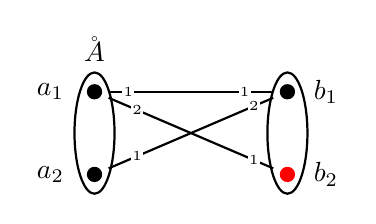
\begin{tikzpicture}[thick,  ncnode/.style={draw=black,,circle,fill=black,scale=0.5},  cnode/.style={draw=red,circle,fill=red,scale=0.5},
  every fit/.style={ellipse,draw,inner sep=-2pt,text width=0.5cm},  -,shorten >= 3pt,shorten <= 3pt, scale=0.7]

% the vertices of A U B
  \node[ncnode] (a1) at (-1,3) {};
  \node[ncnode] (a2) at (-1,1.5) {};
  \node[ncnode] (b1) at (2.5,3) {};
  \node[cnode] (b2) at (2.5,1.5) {};
    \node at (-1.8,3) {$a_1$};
    \node at (-1.8,1.5) {$a_2$};
    \node at (3.2,3) {$b_1$};
    \node at (3.2,1.5) {$b_2$};


% the set A
\node [fit=(a1) (a2),label=above:$\AA$] {};
% the set B
\node [fit=(b1) (b2),label=above:$\BB$] {};

% the edges
\draw(a1) -- (b1) node[pos=0.15,draw=white, fill=white,inner sep=0.1pt] {\textcolor{black}{\tiny 1}} node[pos=0.8,draw=white, fill=white,inner sep=0.1pt] {\textcolor{black}{\tiny 1}};
\draw(a1) -- (b2) node[pos=0.2,draw=white,fill=white,inner sep=0.1pt]{\textcolor{black}{\tiny 2}} node[pos=0.85,draw=white, fill=white,inner sep=0.1pt] {\textcolor{black}{\tiny 1}};
\draw(a2) -- (b1) node[pos=0.2,draw=white,fill=white,inner sep=0.1pt]{\textcolor{black}{\tiny 1}} node[pos=0.85,draw=white, fill=white,inner sep=0.1pt] {\textcolor{black}{\tiny 2}};
\end{tikzpicture}
% % \caption{}
% % \label{subfig:exSMLQ}
% % \end{subfigure}%
% % \begin{subfigure}{.5\textwidth}
% % \centering
% \input{exFig2.tex}
% % \caption{}
% % \label{subfig:exRSMSMTTLQ}
% % \end{subfigure}%
% \caption{\label{subfig:exRSMSMTTLQ} %\label{fig:CexRWSMMM}%
% Red vertices are critical,  black vertices are non-critical. The numbers on the edges denote the ranks of the respective end-points. The instance does not admit any critical stable matching because $b_2$ remains unmatched in each stable matching. $M_1=\{(a_1,b_2),(a_2,b_1),(a_3,b_3)\}$ is critical but not \RWSM\ because the blocking edges $(a_2,b_3)$ and $(a_2,b_4)$ are not justified. $M_2=\{(a_1,b_2),(a_2,b_4),(a_3,b_3)\}$ is \CRWSM\ because the only blocking edge $(a_1,b_1)$ is justified by $a_1$.}
% \end{figure}
 

\begin{figure}
	\begin{center}
		\scalebox{0.8}{\input{exFig2.tex}}
	\end{center}
	\caption{Red vertices are critical,  black vertices are non-critical. The numbers on the edges denote the ranks of the respective end-points. The instance does not admit any critical stable matching because $b_2$ remains unmatched in every stable matching. $M_1=\{(a_1,b_2),(a_2,b_1),(a_3,b_3)\}$ is critical but not \RWSM\ because the blocking edge $(a_2,b_4)$ is not justified. $M_2=\{(a_1,b_2),(a_2,b_4),(a_3,b_3)\}$ is \CRWSM\ because the only blocking edge $(a_1,b_1)$ is justified.}\label{subfig:exRSMSMTTLQ}
\end{figure}


A matching $M$ is called critical relaxed stable matching (\CRWSM) if it is \emph{critical} as well as \emph{relaxed stable}. In the instance shown in Figure~\ref{subfig:exRSMSMTTLQ}, the matching $M_1$ is critical but not \RWSM\ whereas $M_2$ is \CRWSM.

Our first contribution is to show that a \CRWSM\ always exists in our setting. We remark that when $\CC=\emptyset$, an instance of our setting is the same as stable marriage setting with ties but without critical vertices, and hence the set of \CRWSM\ is the same as the set of stable matchings. This immediately implies that computing a maximum size critical \RWSM\ is NP-Hard~\cite{manlove2002hard} and hard to approximate~\cite{halldorsson2007improved}. For the problem of computing a maximum sized stable matching in the presence of two-sided ties, the current best approximation factor \cite{Kiraly13,mcdermid20093,paluch2014faster} is $\frac{3}{2}$. The main result  (Theorem~\ref{theo:main}) provides the same approximation size guarantee for a maximum sized \CRWSM\ in our setting.


 %The main contribution of this work is an efficient algorithm to compute a $\frac{3}{2}$-approximation of a maximum size \CRWSM\ for an instance of our setting.  
\begin{theorem}\label{theo:main}
  Let $G=(\AA\cup\BB,E)$ be an instance of the stable marriage problem with two-sided ties and two-sided critical vertices. Then $G$ always admits a matching $M$ such that $M$ is \CRWSM\ and can be computed efficiently. Moreover, $|M|\ge \frac{2}{3}|M'|$, where $M'$ is a maximum size \CRWSM\ in $G$.  
\end{theorem}


\noindent{\bf Related work:}
As mentioned earlier, the generalizations of the stable marriage problem to allow one of ties in preferences or critical vertices/lower-quota positions has been extensively investigated.
%\cite{manlove2002hard,biro2010popular,hamada2019strategy,NN17,Kavitha2021,NNRS21}. 
The only work which we are aware of allows both ties and critical vertices is a recent work by Goko \etal~\cite{goko2022maximally}. They study the Hospital-Residents problem with lower-quotas with ties on both sides. However, one side of the bipartition cannot have critical vertices. Furthermore, their results are for complete preference, a restricted setting. 
Goko \etal define the maximum satisfaction ratio which for our one-to-one setting coincides with the definition of critical matchings. However, their goal is to compute amongst all stable matchings the one that achieves criticality. %Hence our results are incomparable to theirs.

For strict preferences and lower-quotas / critical vertices, various notions like envyfreeness~\cite{Yokoi20,krishnaa2023envy}, popularity~\cite{NN17,Kavitha2021,NNRS21,nasre2022popular}, and relaxed stability~\cite{krishnaa2020envy,krishnaa2023envy} have been studied. Relaxed stability and popularity do not define the set of matchings even in the one-to-one strict-list setting and critical vertices restricted to one side only (see Appendix~\ref{append:RSvsPop}). Hamada \etal~\cite{HIM16} consider the problem of computing a matching with minimum number of blocking pairs or blocking residents. 

For the stable marriage problem with ties (without critical vertices) there is a long line of investigation \cite{kiraly2011better,mcdermid20093,Kiraly13,paluch2014faster,iwama201425,dean2015factor,huang2015improved} in order to improve the approximation ratio under various restricted settings. The best known approximation algorithm for the case of one-sided ties is by Lam and Plaxton~\cite{lam20191} whereas the best known for the case of two-sided ties is by ~\cite{Kiraly13,mcdermid20093,paluch2014faster}.
We use Kir{\'a}ly's algorithm~\cite{Kiraly13} in our work.

%The notion of \RSM\ was introduced and studied by Krishnaa \etal~\cite{krishnaa2020envy} for \HRLQ\ setting. The authors showed that a critical relaxed stable matching always exists in an \HRLQ\ instance, but computing a maximum-sized relaxed stable matching is NP-hard and hard to approximate below $\frac{21}{19}$. An efficient algorithm for computing a $\frac{3}{2}$-approximation of the maximum size critical relaxed stable matching was also given. 

%Different notions are introduced to deal with the ties in the preference lists and critical vertices. In order to deal with lower quotas in \HRLQ\ problem, Hamada \etal~\cite{HIM16} considered the problem of computing a feasible matching with \emph{minimum} number of blocking pairs or blocking residents -- both these problems turned out to be NP-Hard.  Nasre and Nimbhorkar~\cite{NN17} used the notion of popularity to deal with lower quotas and showed that the maximum cardinality popular matching amongst feasible matchings for an \HRLQ\ problem is efficiently computable. \emph{Envy-freeness}~\cite{wu2018lattice}, a relaxed notion of stability, is another well-investigated optimality notion in \HR\ settings. Yokoi in~\cite{Yokoi20} investigated envy-freeness for \HRLQ\ setting and provided a characterization for \HRLQ\ instances that admit an envy-free matching. %She also gave a linear-time algorithm to compute an envy-free matching, if it exists. 
%Kavitha~\cite{Kavitha2021} and Nasre \etal~~\cite{NNRS21} explored the popularity for two-sided criticality and showed that a maximum size popular matching amongst all critical matchings is efficiently computable.

%Different stable matchings of an instance containing ties can be of different sizes~\cite{irving1994stable}. It is natural to consider the problem of finding a maximum size stable matching. This problem is called \MAXSMTI\ in the literature and is NP-Hard~\cite{iwama1999stable,manlove2002hard}. A $\frac{3}{2}$-approximation algorithm was given by McDermid~\cite{mcdermid20093} and Kir{\'a}ly~\cite{Kiraly13}. Hamada \etal~\cite{hamada2019strategy} studied the tradeoff between strategy-proofness and approximability for the \MAXSMTI\ problem. 

%The closest to our setting is the \emph{marriage model} considered by Goko \etal~\cite{goko2022maximally}. Authors in~\cite{goko2022maximally}, studied \HRLQ\ problem with two-sided ties under four different scenarios. One of the scenarios is the marriage model where ties are allowed on both sides and critical vertices are restricted to one side. This problem has two differences with our setting. Throughout the paper they have assumed that -- (i) the critical vertices are only on one side of bipartition, and (ii) all the preference lists are complete. Thus, our setting is a generalisation of the marriage model considered in~\cite{goko2022maximally}. They studied the problem of computing stable matching with maximum total \emph{satisfaction ratio} for lower quotas, where the satisfaction ratio of each hospital $h$ is given by $\min \{1,\frac{|M(h)|}{q^-(h)}\}$ if $q^-(h)>0$, and 1, otherwise. It is easy to observe that for the marriage model, a matching $M$ has the maximum total satisfaction ratio if and only if it is critical. Also, note that a \emph{stable matching} with maximum total satisfaction ratio may not be critical because an instance may not even admit a critical stable matching. Recall that we are interested in computing a \emph{critical} matching that is {\em optimal}. Thus, although the definitions of critical matching and matching with maximum total satisfaction ratio coincide for the marriage model, the problem considered in~\cite{goko2022maximally} is completely different from ours.



%\noindent{\bf Organisation of the paper:} Section~\ref{sec:prelim} discusses the techniques we use in our algorithm. Algorithm for computing $\frac{3}{2}$-approximation of a maximum size \CRWSM\ is given in Section~\ref{sec:algo}. We prove the correctness of our algorithm in Section~\ref{sec:correct}.% Finally, Section~\ref{sec:conclude} concludes the paper. 
	\section{Preliminaries} \label{sec:prelim}


% If the set of critical nodes $\CC$ is empty for an instance $G$ then $G$ is a stable marriage instance with two-sided ties, and computing a \CRWSM\ for $G$ is the same as computing a stable matching in $G$.  It is well-known that different stable matchings in $G$ have different sizes~\cite{irving1994stable}. Thus, it is natural to consider the problem of computing a maximum size \CRWSM. We represent this problem by \MCRWSM.  Next, we show that if $G$ is an instance of a stable marriage problem with strict preference lists and $\CC\subseteq \BB$ then the Definition~\ref{def:rsm11} and Definition~\ref{def:rsmHRLQ} are equivalent.

% \begin{lemma}\label{lem:equvDef1}
% Let $G$ be an instance of a stable marriage problem with strict preference lists and $\CC\subseteq\BB$. Then a matching $M$ is an \RSM\ according to the Definition~\ref{def:rsm11} if and only if $M$ is an \RSM\ according to the Definition~\ref{def:rsmHRLQ}.
% \end{lemma}

% \begin{proof}
% $\Longrightarrow$  Let $M$ be an \RSM\ according to Definition~\ref{def:rsm11}. If there is no blocking pair w.r.t. $M$ in $G$ then we are done. So, assume that $(a,b)$ is a justified blocking pair w.r.t. $M$ according to Definition~\ref{def:rsm11}. Since no $a\in\AA$ is critical, we claim that the blocking pair $(a,b)$ cannot be justified by condition~\ref{itm:2rwsm}. Suppose $(a,b)$ is justified by condition~\ref{itm:2rwsm} of Definition~\ref{def:rsm11}. Then $b$ is matched in $M$. Since $\CC\subseteq \BB$, it is clear that $M(b)=a'$ is not critical, and hence $a'$ is surplus -- a contradiction that $a$ is not surplus.  Thus, $(a,b)$ is justified by the condition~\ref{itm:1rwsm} of the Definition~\ref{def:rsm11}.  This implies $a$ is matched. That is, all residents participating in the blocking pair are matched. Thus, no unmatched resident blocks $M$. Also, note that $M(a)=b'$ is a critical node and hence cannot be surplus. Thus, the blocking pair $(a,b)$ is acceptable by Definition~\ref{def:rsmHRLQ}. 

% $\Longleftarrow$ Let $M$ be an \RSM\ according to the Definition~\ref{def:rsmHRLQ}. If there is no blocking pair w.r.t. $M$ then we are done. So, let $(a,b)$ be a blocking pair w.r.t. $M$.  Since no unmatched resident participates in a blocking pair, $a$ must be matched.  Note that $b'=M(a)$ is matched in $M$ but not surplus which implies that $b'$ is a critical node. This implies that $a$ is matched and $M(a)$ is a critical node. Thus,  $(a,b)$ is an acceptable blocking pair by Definition~\ref{def:rsm11}. 
% \qed\end{proof}

%  Lemma~\ref{lem:equvDef1} immediately implies that Theorem~4~\cite{krishnaa2023envy} holds for our setting and hence we have Claim~\ref{cl:NPHARD}.
 
% \begin{cl}[Theorem~4~\cite{krishnaa2023envy}]\label{cl:NPHARD}
% The \MCRWSM\ problem for an instance of \SMTTLQ\ is NP-hard and cannot be approximated within a factor of $\frac{21}{19}-\epsilon$ for any $\epsilon >0$ unless $P=NP$.
% \end{cl}

%Given that computing a maximum size critical \RWSM\ is NP-Hard and hard to approximate, we focus on computing a matching with a good approximation to the size of a maximum critical \RWSM. We compute a matching which is $\frac{3}{2}$-approximation to the size of a maximum size \CRWSM. 
Our algorithm described in the next section combines the ideas in 
(i) Kir{\'a}ly's algorithm~\cite{Kiraly13} for computing a stable matching in the presence of two-sided ties and (ii) Multi-level algorithm for computing popular critical matching~\cite{nasre2022popular} for strict preferences.
We give an overview of the algorithms and also define terminology useful for our algorithm.
%Our algorithm is a proposal-based multi-phase, multi-level algorithm where vertices in $\AA$ propose and vertices in $\BB$ accept or reject the proposal. The vertices in $\AA$ propose possibly multiple times,  up to a certain level, as long as they remain unmatched or deficient.  A vertex $b$ which receives the proposal always prefers a higher level vertex  $a$ over any lower level vertex $a'$ irrespective of the ranks of $a$ and $a'$ in $\prefb$. \textcolor{blue}{MN: This does not hold at the t* level, but I guess you do not call it a separate level right? Does this cause confusion? --- Keshav: No I think. Because the first thing is -- I am calling $\T^*$ as a sub-level at level $\T$ and when $\T^*$ is being introduced in our description, I have described the preference ordering in relation to $\T^*$. But, do you feel that it can cause confusion?} Our algorithm is inspired by two different algorithms-- (i) Kir{\'a}ly's algorithm~\cite{Kiraly13} for computing $\frac{3}{2}$-approximation of maximum-sized stable matching in the stable marriage problem with two-sided ties without critical nodes and (ii) maximum-sized popular matching amongst critical matching in the many-to-many setting with two-sided lower-quotas but without ties~\cite{nasre2022popular}. 


\noindent{\bf Overview of Kir{\'a}ly's algorithm~\cite{Kiraly13}.}
 Kir{\'a}ly's algorithm~\cite{Kiraly13} is a proposal-based algorithm where vertices in $\AA$ propose and vertices in $\BB$ accept or reject. We need  the term \emph{uncertain proposal} from \cite{Kiraly13} which is defined below.
 
 \begin{definition}[Uncertain Proposal] \label{def:uncertainProp}
   Let $b$ be some $k^{th}$ rank neighbour of $a$ in $\prefa$. During the course of the algorithm, the proposal from $a$ to $b$ is uncertain if there exists another $k^{th}$ rank neighbour $b'$ of $a$ which is unproposed by $a$ and unmatched in the matching. Once a proposal $(a,b)$ is uncertain, it remains uncertain until $b$ rejects $a$.
\end{definition}
 Each time an  $a\in \AA$ proposes to its \emph{favourite} neighbour $b$ (we define it formally in  Definition~\ref{def:favNbr}), the vertex $b$ accepts/rejects as follows: %(see Definition~\ref{def:favNb).
\begin{enumerate}
    \item If $b$ is unmatched then $b$ immediately accepts the proposal. 
    \item If $b$ is matched, say to $a'$, and $(a',b)$ is an uncertain proposal, then $b$ rejects $a'$ and accepts the proposal from $a$, irrespective of the ranks of $a$ and $a'$ in $\prefb$. In this case, $b$ is {\em marked}
    by $a'$.
    \item If $b$ is matched, say to $a'$, and $(a',b)$ is not an uncertain proposal, then\\ (i) if  $a \succ_b a'$ then $b$ rejects $a'$ and accepts the proposal from $a$, or \\ (ii) if $a' \succeq_b a $ then $b$ rejects $a$.
    \end{enumerate}
    
The reason for $a'$ marking the vertex  $b$ in (2) is as follows:
    %It may happen that $a' \succ_b a$ thus, whenever $a'$ gets rejected by $b$ because of the reason that $a'$ was uncertain about that proposal, the vertex $b$ is \emph{marked} by $a'$. 
    In this case, $b$ rejects the uncertain proposal from $a'$ and accepts $a$ {\em irrespective}
    of the preference of $b'$ between $a$ and $a'$. Later, when $a'$ gets its chance to propose, and if none of the neighbours of $a'$ at the rank of $b$ accept the proposal from  $a'$ then
    %, unproposed neighbour by $a'$ remains at the current rank, 
    $a'$ will propose to the marked vertex $b$ before proposing to the next lower-ranked neighbours.
    In contrast in (3)(i) above, when the proposal $(a', b)$ is not uncertain and $a \succ_b a'$ then $a'$ does not mark $b$. 
    %because $M(b)=a$ is strictly better than $a'$ and $a'$ was not uncertain about the proposal to $b$. 
    Note that a vertex $b\in\BB$ can be part of an uncertain proposal at most once. Once a vertex receives it's first proposal it will remain matched and thereafter cannot be part of any uncertain proposal. Thus, any $b\in\BB$ can be marked at most once during the course of the algorithm.
    
    %If $b$ is matched, say to $a'$, and $a'$ is not uncertain about the proposal, and $a \succ_b a'$ then it rejects $a'$ to get matched with $a$. In this case, $a'$ does not mark $b$ because $M(b)=a$ is strictly better than $a'$ and $a'$ was not uncertain about the proposal to $b$.  If $b$ is matched, say to $a'$, and $(a',b)$ is not an uncertain proposal, and $a' \succeq_b a $ then it rejects $a$. 

Now, we define the favourite neighbour of a vertex $a$, which is an adaptation of the definition in~\cite{Kiraly13}. %in Definition~\ref{def:favNbr}, which uses the concept of \emph{marked} vertices. 
\begin{definition}[Favourite neighbour of $a$] \label{def:favNbr}
  Assume that $k$ is the best rank at which some unproposed or marked neighbours of $a$ exist in $\prefa$. Then $b$ is the favourite neighbour of $a$ if one of the following conditions holds:
    \begin{itemize}
       \item[(i)] there exists at least one unmatched neighbour  of $a$ at the $k^{th}$ rank and $b$ has the lowest index among all such unmatched neighbours, or
        \item[(ii)] all the $k^{th}$-ranked neighbours of $a$ are matched and $b$ is the lowest index among all such neighbours which are unproposed by $a$, or
        \item[(iii)] all the $k^{th}$-ranked neighbours are already proposed by $a$ and $b$ has the lowest index among all the vertices which are marked by $a$.
    \end{itemize}
 \end{definition}

    Kir{\'a}ly's algorithm begins with every vertex $a \in \AA$ being active. As long as there exists an active vertex which is unmatched and has not exhausted its preference list, the vertex proposes to its favourite neighbour.
    If $a\in \AA$ remains unmatched after exhausting its preference list, it achieves a `$*$' status and starts proposing to vertices in $\prefa$ with $*$ status.  The $*$ status of a vertex $a$ can be interpreted as improving the rank of $a$ in $\prefb$ by $0.5$ for any neighbour $b$ of $a$. Thus, the $*$ status vertex is used to decide between vertices in a tie, but does not affect strict preferences.  %A vertex $b\in \BB$ prefers any $*$ status vertex $a$ over a non $*$ status vertex $a'$ if $a=_b a'$. If $a\succ_b a'$ then $*$ status of any of the vertices $a$ or $a'$ does not matter, that is, $b$ prefers $a$ over $a'$ even if $a'$ is $*$ status and $a$ is not $*$ status. A vertex $a\in \AA$ becomes inactive if it is matched or it exhausts its preference list as a $*$ status vertex.
    It is shown in~\cite{Kiraly13} that the resulting matching is a $\frac{3}{2}$-approximation of a maximum size stable matching.



\noindent{\bf Overview of the popular critical matching algorithm~\cite{nasre2022popular}.}
Now, we briefly describe the algorithm in~\cite{nasre2022popular} for computing the maximum size popular critical matching in the one-to-one strict list setting.  Let $\S$ and $\T$ denote the number of critical vertices in $\AA$ and $\BB$, respectively. The algorithm in~\cite{nasre2022popular} is a multi-level algorithm which first matches as many critical vertices from $\BB$ as possible by allowing each unmatched $a\in\AA$ to propose only critical vertices on the $\BB$-side at levels $0,\ldots,\T-1$. At the level $\T$ each vertex $a\in\AA$ is allowed to propose \emph{all} its neighbours. If a vertex $a\in\AA$ remains unmatched even after exhausting its preference list at level $\T$, $a$ raises its level to $\T+1$ and proposes to its neighbours until it is matched or it exhausts its preference list at the level $\T+1$.   If a critical vertex $a$ remains unmatched then $a$ raises its level above $\T+1$ and continues proposing to all its neighbours until it is matched or it exhausts its preference list at the highest level $\S+\T+1$. A vertex $b$ which receives the proposal always prefers a higher level vertex  $a$ over any lower level vertex $a'$ irrespective of the ranks of $a$ and $a'$ in $\prefb$. It is shown in~\cite{nasre2022popular} that the resulting matching is a maximum size popular matching among all the critical matchings.

%\clr{The proofs omitted in the interest of space for $\star$-marked Lemmas  are included in Appendix~\ref{append:proof}.}
	\section{Algorithm for computing \CRWSM} \label{sec:algo}
Our algorithm (see Algorithm~\ref{algo:criRSM}) is a combination of Kir{\'a}ly's algorithm and the popular critical matching algorithm discussed in the previous section. In each level, vertices in $\AA$ propose and vertices in $\BB$ accept or reject. The set of vertices that $a\in \AA$ proposes to depends on its level. Furthermore, depending on the level of $a$, the preference list at that level may be strict or may contain ties. Throughout Algorithm~\ref{algo:criRSM}, $b$ uses its original preference list $\prefb$ which possibly contains ties. For a vertex $a \in \AA$, let $\prefsa$ denote a {\em strict} preference list obtained by breaking ties in $\prefa$ so that the vertices in ties are ordered by increasing order of their indices. Furthermore, let $\prefslqa$ be the strict list obtained from $\prefsa$ by omitting all the non-critical vertices from $\prefsa$.
For example, assume $\prefa = (b_2, b_1), b_5, (b_3, b_4)$ where $b_4$ and $b_5$ are critical vertices. Here, $a$ ranks
$b_1$ and $b_2$ as rank-1, $b_5$ as rank-2 and $b_3$ and $b_4$ as rank-3. We have $\prefsa = b_1, b_2, b_5, b_3, b_4$ and $\prefslqa = b_5, b_4$ where comma separated vertices denote a strict ordering.

%Phase~1 corresponds to fulfilling the deficiencies of the vertices on the $\BB$-side up to the maximum possible extent, phase~2 corresponds to matching the remaining vertices on $\BB$-side and also to increasing the size of the matching, and phase~3 corresponds to fulfilling the deficiencies of the vertices on the $\AA$-side up to the maximum possible extent.  Recall that $\prefa$ and $\prefb$ denote respectively the preference lists of $a\in\AA$ and $b\in\BB$ which may contain ties.  Let $\prefsa$ for $a\in \AA$ denote the preference list obtained by breaking the ties from $\prefa$ in such a way that the vertices in ties are ordered increasingly in their indices. Thus, $\prefsa$ for each $a\in \AA$ is a \emph{strict} preference list. Also, assume that $\prefslqa$ denotes $\prefsa$ restricted to critical nodes. That is, $\prefslqa$ is the strict preference list obtained from $\prefsa$ by omitting all the non-critical nodes from $\prefsa$.


Initially, all the vertices in $\AA$ have their levels set to 0. A vertex $a$ at level $\ell$ is denoted as $a^\ell$.  At a level less than $\T$ (see Line~\ref{alg:all2lqs}--Line~\ref{alg:all2lqe} of Algorithm~\ref{algo:criRSM}), each $a\in\AA$ proposes to vertices in $\prefslqa$. Each time it remains unmatched, it proposes to its \emph{most preferred} neighbour $b$. The most preferred neighbour in $\prefslqa$ or $\prefsa$ is the best-ranked neighbour $b$ to whom $a$ has not yet proposed at the current level. If $a$ remains unmatched after proposing to all its neighbours in $\prefslqa$ at a level $\ell<\T - 1$, then $a$ raises its level to $\ell+1$ and again proposes to vertices in $\prefslqa$. In this part of the algorithm, we invoke \texttt{CriticalPropose()} which encodes the level-based accept/reject by $b$. A vertex $b\in\BB$ prefers $a_i^\ell$  over $a_j^{\ell'}$ if : 
\begin{itemize}
    \item[(i)] either $\ell > \ell'$ (ranks of $a_i$ and $a_j$ in $\prefb$ do not matter) or
    \item[(ii)] $\ell = \ell'$ and $a_i\succ_b a_j$.
\end{itemize} 


\begin{algorithm}[ht]
    \SetKwFunction{deficient}{CriticalPropose}
    \SetKwFunction{tiespropose}{TiesPropose}
    \caption{Critical relaxed stable matching in $G = (\AA \cup \BB, E)$ }\label{algo:criRSM}
    \DontPrintSemicolon
    \SetAlgoLined
    Set $M=\emptyset$, Initialize a queue $Q=\{a^0\ :\ a\in \AA\}$\;
    \While{$Q$ is not empty}{
        Let $a^\ell=dequeue(Q)$ \tcc*{ $a$ is unmatched}
        \If {$\ell<\T$ \label{alg:all2lqs} } { 
            \If{ $a^\ell$ has not exhausted $\prefslqa$}{
               \deficient{$a^\ell,\prefslqa,M,Q$ }\;
            }
            \Else{$\ell=\ell+1$ and add $a^\ell$ to $Q$\; \label{alg:all2lqe}}
        }
        \uElseIf{$\ell==\T$ or $\ell==\T^*$}{  
         \If{$\exists\ b'\in\prefa$ which is marked/unproposed by $a^\ell$ \label{alg:kiralyS}}{   
            % $b=$\favnbr{$a^\ell,\prefa$}\;% \tcc*{ $b$ is the favourite neighbour of $a$}\; 
            \tiespropose{$a^\ell, \prefa, M, Q$}\;
            % Let $b$ be the favourite neighbour of $a$ in $\prefa$ at rank $k$\label{alg:favNbr}\; 
            % \textbf{if} $b$ was marked by $a$ \textbf{then} $a$ unmarks $b$\;
            % \If{$b$ is unmatched}{
            %     $M=M\cup \{(a^\ell,b)\}$\;
            %     \If{there exists an unmatched $b''$ at rank $k$ in $\prefa$ }{
            %         Set $(a^\ell,b)$ as uncertain proposal}
            % }
            % \uElseIf{$b$ is part of an uncertain proposal $(a_j^y,b)$}{
            %     $M=(M\setminus \{(a_j^y,b)\}) \cup \{(a^\ell,b)\}$\;
            %     $a_j^y$ marks $b$ and add $a_j^y$ to $Q$}
            % \uElseIf{$b$ is not part of an uncertain proposal}{
            %     Let $a_j^y= M(b)$\;
            %     \If{$\ell==\T$}{                   
            %         \If{($y<\T$) or (($y==\T$ or $y==\T^*$) and $a\succ_b a_j$)}{
            %             $M=M\setminus \{(a_j^y,b)\}\cup \{(a^\ell,b)\}$ and add $a_j^y$ to $Q$\;}
            %         \Else{add $a^\ell$ to $Q$}
            %     }
            %     \If{$\ell==\T^*$}{                   
            %         \If{($y<\T$) or ($y==\T$ and $a\succeq_b a_j$) or ($y==\T^*$ and $a\succ_b a_j$)}{
            %         $M=M\setminus \{(a_j^y,b)\}\cup \{(a^\ell,b)\}$ and add $a_j^y$ to $Q$\;}
            %         \Else{add $a^\ell$ to $Q$}
            %     }                
            %     }
            }
            \Else{
                \textbf{if} $\ell==\T$ \textbf{then} $\ell=\T^*$ and add $a^\ell$ to $Q$  \label{alg:kiralyE}\;
                \textbf{if} $\ell==\T^*$ \textit{and} $a$ is critical \textbf{then} $\ell=\T+1$ and add $a^\ell$ to $Q$\;
            }
        } 
        \Else{
            \If{$a^\ell$ has not exhausted $\prefsa$ \label{alg:lqToAllS}}{
                \deficient{$a^\ell,\prefsa,M,Q$ }\;
            }
            \Else{ 
                \If{$\ell<\S+\T$ and $a$ is critical \label{alg:lq}}{$\ell=\ell+1$ and add $a^\ell$ to $Q$ \label{alg:lqToAllE}\;}
                 }
        }
    }
    \Return $M$
\end{algorithm}
If vertex $a$ remains unmatched after exhausting $\prefslqa$ at level $\T-1$, $a$ attains level $\T$ where it uses its original preference list $\prefa$ which may contain ties. At level $\T$ our algorithm executes Kir{\'a}ly's algorithm~\cite{Kiraly13}. This corresponds to Line~\ref{alg:kiralyS}--Line~\ref{alg:kiralyE} of Algorithm~\ref{algo:criRSM}. { Kir{\'a}ly's algorithm is encoded in the procedure \texttt{TiesPropose()}.} Since we have two-sided ties at this level, we need the notion of a favourite neighbour and uncertain proposal defined in Section~\ref{sec:prelim}. If the vertex $a$ remains unmatched after exhausting $\prefa$ at level $\T$, it attains the $*$ status, and for this, we have the sub-level $\T^*$. The interpretation of the $*$ status is the same as discussed in Section~\ref{sec:prelim}. %Let $a_i$ and $a_j$ be two neighbours of $b$ in $\prefb$ such that $a_i$ is at level $\T^*$ whereas $a_j$ is at level $\T$. Then $a_i^{\T^*}\succ_b a_j^{\T}$ if and only if $a_i=_b a_j$ or $a_i\succ_b a_j$.

\setlength{\textfloatsep}{8pt}% Remove \textfloatsep
\begin{procedure}
\caption{CriticalPropose($a^\ell,\prefal,M,Q$)}\label{proce:Decide}
    \DontPrintSemicolon
    \SetAlgoLined
    Let $b$ be the most preferred unproposed vertex by $a^\ell$ in $\prefal$ \;
                \If{$b$ is unmatched in $M$}{
                    $M=M\cup \{(a^\ell,b)\}$}
                \Else{
                    Let $a_j^y= M(b)$\;
                    \If{($\ell>y$) or ($\ell==y$ and $a\succ_b a_j$)}{
                    $M=M\setminus \{(a_j^y,b)\}\cup \{(a^\ell,b)\}$ and add $a_j^y$ to $Q$\;
                    }
                    \textbf{else } add $a^\ell$ to $Q$ 
                }
\end{procedure}
If a \emph{critical} vertex $a$ remains unmatched after exhausting its preference list $\prefa$ at level $\T^*$, $a$ raises its level to $\T+1$, and starts proposing to vertices in $\prefsa$ (see Line~\ref{alg:lqToAllS}--Line~\ref{alg:lqToAllE} of Algorithm~\ref{algo:criRSM}). It continues doing so until either it is matched or it has exhausted $\prefsa$ at level $\S+\T$.
In contrast, if a non-critical vertex $a$ remains unmatched after exhausting its preference list $\prefa$ at level $\T^*$, $a$ does not propose any further. 
Recall that $\prefsa$ is a strict preference list containing all the neighbours (not restricted to critical vertices). Here, Algorithm~\ref{algo:criRSM}, again invokes \texttt{CriticalPropose()} for the  level-based accept/reject by $b$. 
%Note that from level 0 to level $\T-1$, a vertex $a\in\AA$ uses its strict preference list restricted to critical vertices, that is $\prefslqa$. This corresponds to Line~\ref{alg:all2lqs}-Line~\ref{alg:all2lqe}.
The algorithm terminates when either (i) all the vertices in $\AA$ are matched or (ii) all unmatched critical $a\in\AA$ have exhausted $\prefsa$ at level $\S+\T$ and all unmatched non-critical $a\in\AA$ have exhausted $\prefa$ at level $\T^*$. %Throughout the algorithm, once a vertex $a$ raises its level, it starts proposing to vertices from the beginning of its current preference list until it is matched. The approach is formally described in Algorithm~\ref{algo:criRSM}. Algorithm~\ref{algo:criRSM} uses a procedure \texttt{CriticalPropose()}. This procedure is the standard accept/reject procedure and is called in phase 1 and phase 2 of our algorithm. Thus, in \texttt{CriticalPropose()} either only critical nodes receive proposals (when $\ell<\T$) or  only critical nodes propose (when $\ell\ge \T+1$). This completes the description of our algorithm. Let $M$ be the output matching of our algorithm. %Algorithm~\ref{algo:criRSM} uses  two procedures \texttt{CriticalProposal()} and \texttt{GetFavNbr()}. The first procedure is the standard accept/reject procedure and is called in phase 1 and phase 2 of our algorithm. Thus, in \texttt{CriticalProposal()} either only critical nodes receive proposals (when $\ell<\T$) or  only critical nodes propose (when $\ell\ge \T+1$). The second procedure \texttt{GetFavNbr()} is used to get the most favourite neighbour of $a$ from the preference list containing ties. Assume $k$ is the best rank at which some unproposed or marked neighbours of $a$ exist in $\prefa$. If there exists an unmatched vertex at rank $k$, then \texttt{GetFavNbr()} returns one such vertex as the favourite neighbour (to ensure that the algorithm behaves deterministically \texttt{GetFavNbr()} chooses the lowest index such vertex). If all vertices at rank $k$ are matched then it returns one which is unproposed by $a$, and if all vertices at rank $k$ are matched and no vertex at rank $k$ remains unproposed by $a$ then it returns one which is marked by $a$.  This completes the description of our algorithm. Let $M$ be the output matching of our algorithm. 
We note that $\S+\T=|\CC|=O(n)$, where $n=|\AA\cup\BB|$ and each edge of $G$ is explored at most $\S+\T+3$ times (at most three times at level $\T$, the Kir{\'a}ly's step, and at most once at every other level). Thus, the running time of our algorithm is $O(n\cdot |E|)$.



%============================================================================================================
%============================================================================================================

% \begin{procedure}%
%     \caption{TiesPropose($a^\ell,\prefal, M, Q$)}\label{proce:TiesProp}
%     \DontPrintSemicolon
%     \SetAlgoLined
%                 Let $b$ be the favourite neighbour of $a$ in $\prefa$ at rank $k$\label{alg:favNbr}\; 
%             \textbf{if} $b$ was marked by $a$ \textbf{then} $a$ unmarks $b$\;
%             \If{$b$ is unmatched}{
%                 $M=M\cup \{(a^\ell,b)\}$\;
%                 \If{there exists an unmatched $b''$ at rank $k$ in $\prefa$ }{
%                     Set $(a^\ell,b)$ as uncertain proposal}
%             }
%             \uElseIf{$b$ is part of an uncertain proposal $(a_j^y,b)$}{
%                 $M=(M\setminus \{(a_j^y,b)\}) \cup \{(a^\ell,b)\}$\;
%                 $a_j^y$ marks $b$ and add $a_j^y$ to $Q$}
%             \uElseIf{$b$ is not part of an uncertain proposal}{
%                 Let $a_j^y= M(b)$\;
%                 \If{$\ell==\T$}{                   
%                     \If{($y<\T$) or (($y==\T$ or $y==\T^*$) and $a\succ_b a_j$)}{
%                         $M=M\setminus \{(a_j^y,b)\}\cup \{(a^\ell,b)\}$ and add $a_j^y$ to $Q$\;}
%                     \textbf{else } add $a^\ell$ to $Q$
%                 }
%                 \If{$\ell==\T^*$}{                   
%                     \If{($y<\T$) or ($y==\T$ and $a\succeq_b a_j$) or ($y==\T^*$ and $a\succ_b a_j$)}{
%                     $M=M\setminus \{(a_j^y,b)\}\cup \{(a^\ell,b)\}$ and add $a_j^y$ to $Q$\;}
%                     \textbf{else } add $a^\ell$ to $Q$
%                 }                
%                 }
% \end{procedure}
% \setlength{\intextsep}{8pt}% Remove \textfloatsep







% \begin{procedure}
% \caption{GetFavNbr($a,\prefa$)}\label{proce:favNbr}
%     \DontPrintSemicolon
%     \SetAlgoLined
%     Let $k$ be the best rank at which some unproposed or marked neighbours of $a$ exist in $\prefa$\;
%     \If{there exists an unmatched neighbour at $k^{th}$ rank}{
%         Let $b$ has the lowest index among all unmatched neighbours at $k^{th}$ rank\;
%     }
%     \uElseIf{there exists an unproposed vertex at $k^{th}$ rank}{
%         Let $b$ has the lowest index among all unproposed neighbours at $k^{th}$ rank\;
%     }
%     \uElseIf{there exists a vertex at $k^{th}$ rank which is marked by $a$}{
%         Let $b$ has the lowest index among all the marked neighbours by $a$ at $k^{th}$ rank\;
%     }
%     return $b$\;
% \end{procedure}



% \begin{algorithm}
%     \SetKwFunction{favnbr}{GetFavNbr}
%     \caption{Critical relaxed stable matching in $G = (\AA \cup \BB, E)$ }\label{algo:criRSMOld}
%     \DontPrintSemicolon
%     \SetAlgoLined
%     Set $M=\emptyset$, Initialize a queue $Q=\{a^0\ :\ a\in \AA\}$\;
%     \While{$Q$ is not empty}{
%         Let $a^\ell=dequeue(Q)$ \tcc*{ $a$ is unmatched}
%         \If {$\ell<\T$ \label{alg:all2lq} } { 
%             \If{ $a^\ell$ has not exhausted $\prefslqa$}{
%                 Let $b$ be the most preferred unproposed vertex by $a^\ell$ in $\prefslqa$ \;
%                 \textbf{if} $b$ is unmatched \textbf{then} $M=M\cup \{(a^\ell,b)\}$\;
%                 \Else{
%                     Let $a_j^y= M(b)$\;
%                     \If{($\ell>y$) or ($\ell==y$ and $a\succ_b a_j$)}{
%                     $M=M\setminus \{(a_j^y,b)\}\cup \{(a^\ell,b)\}$ and add $a_j^y$ to $Q$} \label{dec:st2}
%                 }
%             }
%             \Else{$\ell=\ell+1$ and add $a^\ell$ to $Q$\;}
%         }
%         \uElseIf{$\ell==\T$ or $\ell=\T^*$}{  
%          \If{there exists a marked/unproposed vertex by $a^\ell$ in $\prefa$}{   
%            $b=$\favnbr{$a^\ell,\prefa$}\; 
%             \textbf{if} $b$ is marked by $a$ previously \textbf{then} $a$ unmarks it\;
%             \textbf{if} $b$ is unmatched \textbf{then} $M=M\cup \{(a^\ell,b)\}$\;
%             \uElseIf{$b$ is matched and is part of an uncertain proposal $(a_j^y,b)$}{$M=(M\setminus \{(a_j^y,b)\}) \cup \{(a^\ell,b)\}$, $b$ is marked by $a_j$ and $a_j^y$ is added to $Q$}
%             \uElseIf{$b$ is matched and is not part of an uncertain proposal}{
%                 Let $a_j^y= M(b)$\;
%                 \If{$\ell==\T$}{                   
%                     \If{($\ell>y$) or ($y==\T$ and $a\succ_b a_j$)}{
%                     $M=M\setminus \{(a_j^y,b)\}\cup \{(a^\ell,b)\}$ and add $a_j^y$ to $Q$\;}
%                 }
%                 \If{$\ell==\T^*$}{                   
%                     \If{($y< \T$) or ($\ell==y$ and $a\succ_b a_j$) or ($y== \T$ and $a =_b a_j$)}{
%                     $M=M\setminus \{(a_j^y,b)\}\cup \{(a^\ell,b)\}$ and add $a_j^y$ to $Q$\;}
%                 }
                
%                 }
%             }
%             \Else{
%                 \textbf{if} $\ell==\T$ \textbf{then} $\ell=\T^*$\;
%                 \textbf{if} $\ell==\T^*$ \textit{and} $a$ is deficient \textbf{then} $\ell=\T+1$\;
%             }
%         } 
%         \Else{
%             \If{$a^\ell$ has not exhausted $\prefsa$}{
%                 Let $b=$ the most preferred unproposed vertex by $a^\ell$ in $\prefsa$\;
%                 \textbf{if} $b$ is unmatched \textbf{then} $M=M\cup \{(a^\ell,b)\}$\;
%                 \Else{
%                     Let $a_j^y= M(b)$\;
%                     \If{($\ell>y$) or ($\ell==y$ and $a\succ_b a_j$)}{
%                     $M=M\setminus \{(a_j^y,b)\}\cup \{(a^\ell,b)\}$ and add $a_j^y$ to $Q$}
%                 }
%             }
%             \Else{ 
%                 \If{$\ell<\S+\T$ and $a$ is deficient \label{alg:lq}}{$\ell=\ell+1$ and add $a^\ell$ to $Q$ \label{alg:lq1}\;}
%                  }
%         }
%     }
%     \Return $M$
% \end{algorithm}


	\section{Correctness of our algorithm} \label{sec:correct}

We prove that the matching $M$ output by Algorithm~\ref{algo:criRSM} is 
\begin{enumerate} [(I)]
    \item  Critical as well as relaxed stable (\RWSM) and
    \item  A $\frac{3}{2}$ approximation to the maximum size $\CRWSM$ in $G$.
\end{enumerate}
The proofs of claims marked with $\star$ are deferred to Appendix.

%Our correctness proof involves showing that the matching $M$ is -- (i) critical, (ii) relaxed stable and  (iii) $\frac{3}{2}$-approximation to the maximum size $\CRWSM$ in an instance $G$ of the \SMTTLQ\ problem
The partition of vertices defined below based on the levels of vertices in $\AA$ and the matching $M$ is useful for us. 
%In order to prove the correctness, we partition the vertices of $\AA\cup\BB$ into subsets and establish some properties about these sets. 

%\vspace{0.1in}


\noindent \textbf{Partition of vertices:} 
%We partition the vertex set $\AA\cup\BB$ as described next. 
The vertex set $\AA$ is partitioned into $\AA_0\cup\AA_1\cup\ldots\cup\AA_{\T}\cup\ldots\cup\AA_{\S+\T}$, and the vertex set $\BB$ is partitioned into $\BB_0\cup\BB_1\cup\ldots\cup\BB_{\T}\cup\ldots\cup\BB_{\S+\T}$. For every matched vertex $a\in\AA$ there exists $x\in\{0,\ldots,\S+\T\}$ such that $(a^x,b)\in M$. We use $x$ to partition the vertex set. Note that if  $(a^{\T^*},b)\in M$ then for the purpose of partitioning we consider $\T^*=\T$  as $\T^*$ is a sub-level of the level $\T$.
\begin{itemize}
    \item \label{itm:part111} \textbf{Matched vertices in $\AA\cup \BB$:} Let $a\in \AA, b\in \BB$ and $(a^x,b)\in M$ for some $x\in\{0,\ldots,\S+\T\}$. Then we add $a$ to $\AA_x$ and $b$ to $\BB_x$.

    \item \label{itm:part411}{\bf Unmatched vertices in $\AA\cup\BB$:} 
    \begin{itemize}
        \item If a non-critical vertex $a\in \AA$ is unmatched in $M$ then we add $a$ to $\AA_{\T}$.
        \item If a critical vertex $a\in \AA$ is unmatched in $M$ then we add $a$ to $\AA_{\S+\T}$.
    % \end{itemize}



    
    % \item \label{itm:part5}\textbf{Unmatched vertices in $\BB$:}
    % \begin{itemize}
        \item If a non-critical vertex $b\in \BB$ is unmatched in $M$ then we add $b$ to $\BB_{\T}$.
        \item If a critical vertex $b\in \BB$ is unmatched in $M$ then we add $b$ to $\BB_0$.
        %=====================================================================================================
%=====================================================================================================

\begin{procedure}%
    \caption{TiesPropose($a^\ell,\prefal, M, Q$)}\label{proce:TiesProp} %( Kir{\'a}ly's algorithm~\cite{Kiraly13})
    \DontPrintSemicolon
    \SetAlgoLined
                Let $b$ be the favourite neighbour of $a$ in $\prefa$ at rank $k$\label{alg:favNbr}\; 
            \textbf{if} $b$ was marked by $a$ \textbf{then} $a$ unmarks $b$\;
            \If{$b$ is unmatched}{
                $M=M\cup \{(a^\ell,b)\}$\;
                \If{there exists an unmatched $b''$ at rank $k$ in $\prefa$ }{
                    Set $(a^\ell,b)$ as uncertain proposal}
            }
            \uElseIf{$b$ is part of an uncertain proposal $(a_j^y,b)$}{
                $M=(M\setminus \{(a_j^y,b)\}) \cup \{(a^\ell,b)\}$\;
                $a_j^y$ marks $b$ and add $a_j^y$ to $Q$}
            \uElseIf{$b$ is not part of an uncertain proposal}{
                Let $a_j^y= M(b)$\;
                \If{$\ell==\T$}{                   
                    \If{($y<\T$) or (($y==\T$ or $y==\T^*$) and $a\succ_b a_j$)}{
                        $M=M\setminus \{(a_j^y,b)\}\cup \{(a^\ell,b)\}$ and add $a_j^y$ to $Q$\;}
                    \textbf{else } add $a^\ell$ to $Q$
                }
                \If{$\ell==\T^*$}{                   
                    \If{($y<\T$) or ($y==\T$ and $a\succeq_b a_j$) or ($y==\T^*$ and $a\succ_b a_j$)}{
                    $M=M\setminus \{(a_j^y,b)\}\cup \{(a^\ell,b)\}$ and add $a_j^y$ to $Q$\;}
                    \textbf{else } add $a^\ell$ to $Q$
                }                
                }
\end{procedure}
\setlength{\intextsep}{8pt}% Remove \textfloatsep

%===============================================================================================================
%===============================================================================================================

    \end{itemize}
\end{itemize}



It is convenient to visualize the partitions as shown in Figure~\ref{fig:maxlevelgraph11}. This particular drawing of the graph $G$ is denoted by $G_M$ throughout the rest of the section. It is useful to assume that the edges in $G_M$ are implicitly directed from $\AA$ to $\BB$. By construction, the edges of $M$ (shown in blue colour) are horizontal whereas the unmatched edges (shown as solid black edges) can be horizontal, upwards or downwards.  

We state the properties of the vertices and edges in $G_M$ with respect to this partition in Property~\ref{property:GM}. % which is justified in the appendix.  
We briefly justify the properties in Property~\ref{property:GM} as follows. Only critical vertices in $\AA$ attain levels above $\T$. This implies that the partition set $\AA_{\T+1},\ldots,\AA_{\S+\T}$ contain only critical $a\in\AA$. Thus, we have Property~\ref{property:GM}(\ref{obs:partitionPorp2}).
Since each $a\in\AA$ at a level at most $\T-1$ does not propose to any non-critical vertex, the matched partner of each $a^x$ for $x\le \T-1$ is a critical vertex. Also, all the unmatched non-critical vertices on $\BB$-side are only in $\BB_{\T}$. This implies that the partition set $\BB_0,\ldots,\BB_{\T-1}$ contain only critical $b\in\BB$.  Thus, we have Property~\ref{property:GM}(\ref{obs:partitionPorp1}). 
 If a vertex $a$ remains unmatched in $M$ then by the design of our algorithm it must have exhausted its preference list at level $\S+\T$ (if it is a critical vertex) or at level $\T$, more specifically $\T^*$, (if it is a non-critical vertex)  and got rejected by each of its neighbours. Recall that each $b$ prefers a higher level $a$ over any lower level $a'$ irrespective of the ranks of $a$ and $a'$ in $\prefb$. Thus, Property~\ref{property:GM}(\ref{obs:partitionPorp4}) and Property~\ref{property:GM}(\ref{obs:partitionPorp3}) hold in $G_M$. Observe that if any vertex $b\in\BB$ receives a proposal then it cannot remain unmatched in $M$. This implies, if a critical $b$ is unmatched then none of its neighbours has proposed it at level 0, which further implies that they have not exhausted $\prefslqa$ at level 0. By construction, $b$ is in $\BB_0$. Hence, we have Property~\ref{property:GM}(\ref{obs:partitionPorp5}). Similarly, if $b$ is non-critical and unmatched then none of its neighbours can go to level $\T+1$ or above. By construction, $b$ is in $\BB_{\T}$. Hence, we have Property~\ref{property:GM}(\ref{obs:partitionPorp6}).

% Since each $a\in\AA$ at a level at most $\T-1$ proposes to vertices in $\prefslqa$ and only deficient $a$ raises its level above $\T$. The above partition and the matching $M$ implies that the partition set $\BB_0,\ldots,\BB_{\T-1}$ contain only critical $b\in\BB$ and all non-critical $b\in\BB$ are in $\BB_{x}$ for $x\ge \T$. Similarly, the partition set $\AA_{\T+1},\ldots,\AA_{\S+\T}$ contain only critical $a\in\AA$ and all non-critical $a\in\AA$ are in $\AA_{x}$ for $x\le \T$. Thus, we have Property~\ref{property:GM}(\ref{obs:partitionPorp1}) and Property~\ref{property:GM}(\ref{obs:partitionPorp2}). If a vertex $a$ remains unmatched in $M$ then by the design of our algorithm it must have exhausted its preference list at level $\T$, more specifically $\T^*$, (if it is a non-critical node) or at level $\S+\T$ (if it is a critical node) and got rejected by each of its neighbours. Recall that each $b$ prefers a higher level $a$ over any lower level $a'$ irrespective of the ranks of $a$ and $a'$ in $\prefb$. Thus, Property~\ref{property:GM}(\ref{obs:partitionPorp3}) and Property~\ref{property:GM}(\ref{obs:partitionPorp4}) hold in $G_M$. Observe that if any vertex $b\in\BB$ receives a proposal then it cannot remain unmatched in $M$. This implies that an unmatched $b$ did not receive any proposal. Thus, we have Property~\ref{property:GM}(\ref{obs:partitionPorp5}) and Property~\ref{property:GM}(\ref{obs:partitionPorp6}).


\begin{figure}
\begin{center}
    \scalebox{0.8}{
	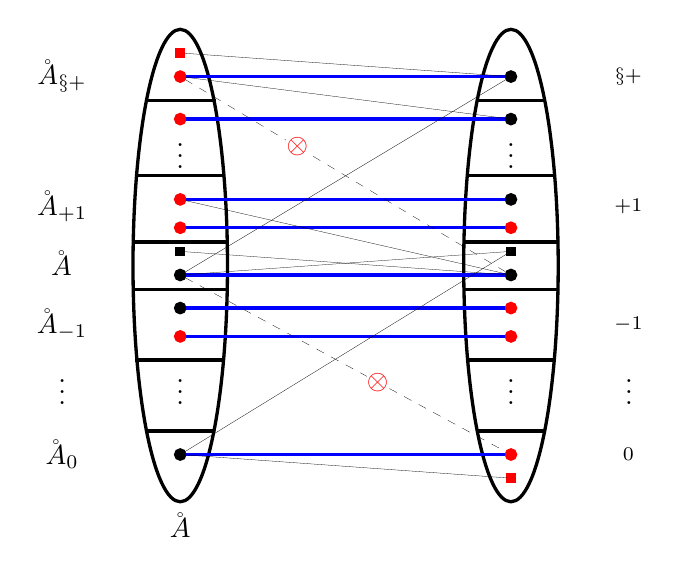
\begin{tikzpicture}[scale=0.6, thick,fsnode/.style={draw,circle,fill=black,scale=0.4}, lnode/.style={draw=red,circle,fill=red,scale=0.4}, snode/.style={draw=blue,circle,fill=blue,scale=0.4},tnode/.style={draw=black,fill=black,scale=0.4}, ltnode/.style={draw=red,fill=red,scale=0.4}]
	% ----------------A0'--------------------%
	\draw[very thick] (1,1.5) ellipse (1cm and 5cm);
	\node at (1,-4) {$\AA$};
	\draw[very thick] (0.25,5) -- (1.75,5);
	\node at (1,4) {\vdots};
	\draw[very thick] (0.07,3.4) -- (1.93,3.4);
	\draw[very thick] (0,2) -- (2,2);
	\draw[very thick] (0,1) -- (2,1);
	\node at (1,-1) {\vdots};
	\draw[very thick] (0.05,-0.5) -- (1.95,-0.5);
	\draw[very thick] (0.3,-2) -- (1.7,-2);
	\node at (-1.5,5.5) {$\AA_{\S+\T}$};
	\node at (-1.5,2.75) {$\AA_{\T+1}$};
	\node at (-1.5,1.5) {$\AA_{\T}$};
	\node at (-1.5,0.25) {$\AA_{\T-1}$};
	\node at (-1.5,-1) {\vdots};
	\node at (-1.5,-2.5) {$\AA_{0}$};
% 	% -------------B0'--------------%
	\draw[very thick] (8,1.5) ellipse (1cm and 5cm);
	\node at (8,-4) {$\BB$};
	\draw[very thick] (7.25,5) -- (8.75,5);
	\node at (8,4) {\vdots};
	\draw[very thick] (7.07,3.4) -- (8.93,3.4);
	\draw[very thick] (7,2) -- (9,2);
	\draw[very thick] (7,1) -- (9,1);
	\node at (8,-1) {\vdots};
	\draw[very thick] (7.05,-0.5) -- (8.95,-0.5);
	\draw[very thick] (7.3,-2) -- (8.7,-2);
	\node at (10.5,5.5) {$\BB_{\S+\T}$};
	\node at (10.5,2.75) {$\BB_{\T+1}$};
	\node at (10.5,1.5) {$\BB_{\T}$};
	\node at (10.5,0.25) {$\BB_{\T-1}$};
	\node at (10.5,-1) {\vdots};
	\node at (10.5,-2.5) {$\BB_0$};
% 	% ----------matched edges--------------%  
	\node[fsnode] (b3) at (8,5.5) {};
	\node[lnode] (a4) at (1,5.5) {};
	\draw[very thick,blue] (a4) -- (b3);
	\node[lnode] (a5) at (1,4.6) {};
	\node[fsnode] (b4) at (8,4.6) {};
    \draw[very thick,blue] (a5) -- (b4);
    \node[fsnode] (a2) at (1,0.6) {};
	\node[lnode] (b2) at (8,0.6) {};
	\draw[very thick,blue] (a2) -- (b2);
    \node[lnode] (a10) at (1,0) {};
	\node[lnode] (b10) at (8,0) {};
	\draw[very thick,blue] (a10) -- (b10);
    \node[lnode] (a9) at (1,2.9) {};
	\node[fsnode] (b9) at (8,2.9) {};
    \draw[very thick,blue] (a9) -- (b9);
    \node[lnode] (a11) at (1,2.3) {};
	\node[lnode] (b11) at (8,2.3) {};
    \draw[very thick,blue] (a11) -- (b11);
	\node[fsnode] (a6) at (1,1.3) {};
	\node[fsnode] (b5) at (8,1.3) {};
	\draw[very thick,blue] (a6) -- (b5);
	\node[fsnode] (a8) at (1,-2.5) {};
	\node[lnode] (b8) at (8,-2.5) {};
	\draw[very thick,blue] (a8) -- (b8);
	\node[ltnode] (b6) at (8,-3) {};
	\node[ltnode] (a1) at (1,6) {};
	\node[tnode] (b7) at (8,1.8) {};
	\node[tnode] (a7) at (1,1.8) {};
% 	%------------other edges---------------%  
	\draw[ultra thin] (a4) -- (b4);
	\draw[ultra thin] (a6) -- (b3);
	\draw[ultra thin] (a6) -- (b7);
	\draw[ultra thin] (a7) -- (b5);
	\draw[ultra thin] (a8) -- (b6);
	\draw[ultra thin] (a1) -- (b3);
    \draw[ultra thin] (a8) -- (b7);
    \draw[ultra thin] (a9) -- (b5);
	
% 	%------------invalid edges-------------%  
    
    
\draw[ultra thin, dashed] (a4) -- (b5)node[pos=0.35,fill=white,inner sep=0.1pt]{\textcolor{red}{$\otimes$}};
\draw[ultra thin, dashed] (a6) -- (b8)node[pos=0.6,fill=white,inner sep=0.1pt]{\textcolor{red}{$\otimes$}};
    
% \draw[ultra thin, dashed] (a3) -- (b4)node[pos=0.73,fill=white,inner sep=0.1pt]{\textcolor{red}{$\otimes$}};
	\end{tikzpicture}}
\end{center}
\caption{The graph $G_M$. Red vertices are critical and black vertices are non-critical. Matched vertices are represented by circles and unmatched vertices are represented by squares. The blue horizontal lines represent matched edges in $M$. Solid black lines represent edges which are not matched in $M$. Dashed black lines marked with crossed red circles represent steep downward edges that are not present in $G_M$ (Lemma~\ref{pr:noedge11}).
}
\label{fig:maxlevelgraph11}
\end{figure}

\vspace{-0.1in}

\begin{property}\label{property:GM}
Let $a\in\AA$ and $b\in\BB$. Then the following hold in graph $G_M$.
\begin{enumerate}
    \item \label{obs:partitionPorp2} If $a\in \bigcup_{x=\T+1}^{\T+\S}\AA_x$ then $a$ is critical. Thus, $|\bigcup_{x=\T+1}^{\T+\S}\AA_x|\le \S$.
    \item \label{obs:partitionPorp1} If $b\in \bigcup_{x=0}^{\T-1}\BB_x$ then $b$ is critical. Thus, $|\bigcup_{x=0}^{\T-1}\BB_x|\le \T$.
    \item \label{obs:partitionPorp4} If $a$ is critical and is unmatched in $M$ then $a\in \AA_{\S+\T}$ and all the neighbours of $a$ are matched and present in $\BB_{\S+\T}$ only.
    \item \label{obs:partitionPorp3} If $a$ is not critical and is unmatched in $M$ then $a\in \AA_{\T}$ and all the neighbours of $a$ are matched and present in $\BB_{x}$ for $x\ge \T$.    
    \item \label{obs:partitionPorp5} If $b$ is critical and is unmatched in $M$ then $b\in \BB_{0}$ and all the neighbours of $b$ are present in $\AA_{0}$ only.
    \item \label{obs:partitionPorp6} If $b$ is  not critical and is unmatched in $M$ then $b\in\BB_{\T}$ and all the neighbours of $b$ are present in $\AA_{x}$ for $x\le \T$.
    
\end{enumerate}
\end{property}


Let $(a, b)\in E$ be  an edge such that $a \in \AA_x$ and $b\in \BB_y$. We say that such an edge is of the form $\AA_x \times \BB_y$.  Lemma~\ref{pr:noedge11} below gives an important property about the edges which cannot be present in $G_M$. An edge of the from $\AA_x \times  \BB_y$ with $x>y+1$ is referred to as a \emph{steep downward} edge.

\begin{lemma}\label{pr:noedge11}
The graph $G_M$ does not contain steep downward edges. That is, there is no edge in $G_M$ of the form
$\AA_x \times  \BB_y$ such that $x>y+1$.
\end{lemma}
\begin{proof}
Let $(a,b)$ be any edge in $G_M$.  If $b$ is unmatched then irrespective of whether $b$ is critical or not by Property~\ref{property:GM}(\ref{obs:partitionPorp5}) and Property~\ref{property:GM}(\ref{obs:partitionPorp6}), we have $x\le y$. Now suppose $(a',b)\in M$. If $a=a'$ then by construction of $G_M$, $(a,b)\in\AA_x \times  \BB_x$ for some $x\in\{0,\ldots,\S+\T\}$.  If $a\not=a'$ then we use the following claim (Claim~\ref{lem:noedge11}). It is immediate from this claim that $b$ is in $\BB_z$ for $z\ge x-1$.
\begin{cl}\label{lem:noedge11}
Let  $(a,b)\in E\setminus M$ and $b$ be matched in $M$ to $\Tilde{a}$ at level $y$, that is, $M(b)=\Tilde{a}^y$. If the level $x$ of $a$ is at least 2 then $y\ge x-1$.
\end{cl} 
\noindent \emph{Proof of Claim~\ref{lem:noedge11}: }
  Suppose for contradiction that there exists $\Tilde{a}\in \AA$ such that $(\Tilde{a}^y,b)\in M$ for $y<x-1$. The fact that $(a,b)\in E$ and $a$ achieves the level $x$ implies that $a$ remains unmatched after $a^{x-1}$ exhausted its preference list $\prefa$, $\prefsa$ or $\prefslqa$ as appropriate.  Note that if $b$ receives a proposal from a vertex $\Tilde{a}\in\AA$ at levels below $x-1$ then $b$ is also available to receive proposals from vertices in $\AA$ at levels $\ge x-1$. This is because when a vertex in $\AA$ transitions to a higher level, it proposes to possibly a superset of vertices that it proposes to in the lower level (recall that $\prefa$ and $\prefsa$ is a superset of $\prefslqa$). Furthermore, if a vertex in $\BB$ receives a proposal from some $a'\in \AA$ at a level $z$ then it is available to receive a proposal from all its neighbours proposing at level $z$.

Since $b$ is matched to a vertex at level $y<x-1$, it must be the case that $b$ has received a proposal from $a^{x-1}$ and it accepted this proposal by rejecting $\Tilde{a}^y$ because $y<x-1$. Recall that a vertex $b\in\BB$ always prefers $a$ over $\Tilde{a}$ if $a$ is at a higher level than that of $\Tilde{a}$. Thus, $(a,b)\in M$ and we get a contradiction to the fact that $(a,b)\notin M$.  \qed
This completes the proof of Lemma~\ref{pr:noedge11}. \qed
\end{proof}


% \begin{lemma}\label{lem:BPUpward}
% Let $(a,b)\in E\setminus M$ and $b\succ_a M(a)$ and $a\succ_b M(b)$. Then the edge $(a,b)$ is of the form $\AA_x \times  \BB_y$ such that $x<y$  in $G_M$. That is, each blocking edge in $G_M$ is an upward edge.
% \end{lemma}

\begin{lemma}\label{lem:BPUpward}
Let $(a,b)$ be a blocking pair w.r.t. $M$.  Then the corresponding edge in $G_M$ is an upward edge.
\end{lemma}
\begin{proof}
For the blocking pair $(a,b)$ let $a$ and $b$ be at levels $x$ and $y$, respectively. First, suppose that $b$ is a critical vertex. Since $(a,b)$ is a blocking pair, irrespective of whether $a$ is matched or unmatched, $a^x$ must have proposed to critical $b$. Thus, $b$ cannot remain unmatched. Thus, $M(b)$ exists. Since $(a,b)\notin M$, it must be the case that $b$ rejected $a^x$. The fact that $a \succ_b M(b)$ and $b$ rejected $a^x$ implies that $M(b)$ is at a level $y>x$. Thus, the $(a,b)$ edge is an upward edge in $G_M$. 

Now, suppose that $b$ is a non-critical vertex. Then by the construction of $G_M$, $b\in\BB_y$ for $y\ge \T$. If $x<\T$ then we are done. So, assume that $x\ge \T$. Since $x\ge \T$, $a^x$ is allowed to propose to \emph{all} of its neighbours. Again, since $(a,b)$ is a blocking pair, irrespective of whether $a$ is matched or unmatched, $a^x$ must have proposed $b$.  Thus, $M(b)$ exists. Since $(a,b)\notin M$, $b$ rejected $a^x$ for $x\ge \T$. The fact that $a\succ_b M(b)$ implies $M(b)$ must be at a level $y$ such that $y>x$. Thus, $(a,b)$ edge is an upward edge in $G_M$. 
\qed\end{proof}



Now, we show that the matching $M$ output by Algorithm~\ref{algo:criRSM} is critical. To prove the criticality of $M$, we use a property of an arbitrary critical matching $N$ which is given in Claim~\ref{lem:noLessDef}. Basically, Claim~\ref{lem:noLessDef} states that no matching matches more critical vertices from a particular side $\AA$ or $\BB$ than a critical matching. In other words, the number of critical vertices matched from $\AA$-side or $\BB$-side is optimum in any critical matching. This also implies that the number of critical vertices matched from $\AA$-side or $\BB$-side is invariant across all critical matchings. 
That is, if a critical matching $M_1$ matches $p$ number of critical vertices from $\AA$ and $q$ number of critical vertices from $\BB$ then any other critical matching, say $M_2$, also matches $p$ many critical vertices from $\AA$ and $q$ many critical vertices from $\BB$. This claim is similar to the one in~\cite{nasre2022popular}.

\begin{cl}\label{lem:noLessDef}
Let $N$ be any critical matching and $M$ be any matching in $G$. Then the number of critical vertices matched in $N$ from $\AA$ is at least the number of critical vertices matched in $M$ from $\AA$. Similarly, the number of critical vertices matched in $N$ from $\BB$ is at least the number of critical vertices matched in $M$ from $\BB$.
\end{cl}
\begin{proof}
Here we will prove the first statement, that is, we show that the number of critical vertices matched in a critical matching $N$ from $\AA$ is at least the number of critical vertices matched in any matching $M$ from $\AA$. The proof for the second statement is symmetric. 


Consider the symmetric difference $N\oplus M$.  Suppose for contradiction that $N$ matches strictly less number of critical vertices from $\AA$ than that of $M$.  This implies there must exist a maximal alternating path $\rho=\langle u,u'\ldots,v\rangle$ starting at an unmatched critical vertex $u\in\AA$ in $N$ such that using $\rho$ we obtain a matching $N'=N\oplus \rho$ which matches strictly more number of critical vertices from $\AA$ than $N$ on $\rho$.  Note that $\rho$ is a maximal $M$-$N$ alternating path starting with an $M$ edge $(u,u')$ such that critical $u$ is unmatched in $N$ but matched in $M$. We consider the two cases below depending on the parity of the length of $\rho$.

If $\rho$ is of odd length then it is an augmenting path with respect to $N$. That is, critical $u$ becomes matched in $N'$ from unmatched in $N$  whereas the matched/unmatched status of all other vertices on $\rho$, except $v$, remains the same as in $N$. Note that $\rho$ is an augmenting path for $N$ and hence $v$ gets matched in $N'$ from unmatched in $N$.  Thus, $N'$ matches more number of critical vertices from $\AA$ than that of $N$. Also, note that all the vertices from $\BB$, except $v$, remain matched/unmatched as they were in $N$. That is, the number of matched critical vertices from $\BB$ either increases by 1 (when $v$ is critical) or remains the same. Thus $N'$ matches more number of critical vertices overall than that of a critical matching $N$ -- a contradiction. 

If $\rho$ is of even length then due to the maximality of $\rho$, the other endpoint $v\in\AA$ is unmatched in $M$ and hence, $\rho$ ends with an $N$-edge. Note that $v\in\AA$ is unmatched in $M$ and $u$ is critical but matched in $M$. If $v$ is a critical vertex then the number of critical vertices matched in $N'$ and $N$ remain the same. This contradicts the selection of our path $\rho$. Recall $\rho$ is an alternating path such that $N'=N\oplus \rho$ matches strictly more number of critical vertices from $\AA$. Thus, $v$ is not a critical vertex. But then the number of critical vertices matched in $N'$ is strictly less than that of $N$. This contradicts the selection of our path $\rho$.

 Thus, we conclude that such a path $\rho$ does not exist and hence the number of critical vertices matched in $N$ from $\AA$ is at least the number of critical vertices matched in $M$ from $\AA$.\qed
 \end{proof}


\begin{lemma}\label{lem:critical11}
The output matching $M$ is critical for $G$.
\end{lemma}
% \noindent\textit{Proof sketch:}
% We prove the criticality of $M$ by using the level structure of the graph $G_{M}$. The idea is to show that there is no alternating path $\rho$ in $G_M$ with respect to $M$ such that the number of critical vertices matched in  $M\oplus \rho$ is more than the number of critical vertices matched in $M$. We prove the criticality for the individual parts, that is, for $\AA$-part and for $\BB$-part. For the $\AA$-part we show that the path $\rho$ begins at the highest level $\S+\T$, has at least the first two vertices on the $\AA$-side at the same level and the other end at a level below $\T+1$. Thus, the number of vertices in $\AA$ along this path is at least $\S+1$. We further show that all these vertices (at least $\S+1$) from $\AA$ must lie in levels $\T+1, \ldots, \S+\T$, which contradicts Property~\ref{property:GM}(\ref{obs:partitionPorp2}). \qed
\begin{proof}
We prove the criticality of $M$ by using the level structure of the graph $G_{M}$. The idea is to show that there is no alternating path $\rho$ in $G_M$ w.r.t. $M$ such that $M\oplus \rho$ results in more critical vertices matched than in $M$. We prove the criticality in two parts. First, we prove ($\AA$-part) where we show that $M$ matches the maximum possible critical vertices from the set $\AA\cap\CC$ and then we prove ($\BB$-part) where we show that $M$ matches the maximum possible critical vertices from the set $\BB\cap\CC$. Thus, by using Claim~\ref{lem:noLessDef} above, we conclude that $M$ is critical. Let $N$ be any critical matching in $G$.


\vspace{0.1in}


\noindent \textbf{Proof of ($\AA$-part):} Suppose for contradiction that $M$ does not match the maximum possible critical vertices from the set $\AA\cap\CC$. This implies that there exists an alternating path $\rho$ in $M\oplus N$ such that $N$ matches more critical vertices from $\AA$ on $\rho$ than in $M$. Let $\rho=\langle u_0, v_1, u_1, v_2, u_2, \ldots, v_k, u_k,\ldots \rangle$ where $(v_i,u_i)\in M$ and the other edges of $\rho$ are in the matching $N$. Furthermore, assume that the first vertex $u_0$ represents a vertex $a\in\AA$ such that critical $a$ is matched in $N$ but unmatchedy in $M$. Since critical $a$ is unmatched in $M$, by Property~\ref{property:GM}(\ref{obs:partitionPorp4}), $a\in\AA_{\S+\T}$. Thus, $\rho$ starts at level $\S+\T$ in $G_M$, that is, $u_0\in\AA_{\S+\T}$. Since $u_0=a$ is critical and unmatched in $M$, by Property~\ref{property:GM}(\ref{obs:partitionPorp4}), $v_1\in\AA_{\S+\T}$ and $u_1=M(v_1)$ is in $\AA_{\S+\T}$. The other end of $\rho$ can be in $\AA$ or in $\BB$. We consider both these cases below.

\noindent\textbf{The path $\rho$ ends at a vertex in $\AA$:} Suppose that the path ends at a vertex in $\AA_x$ for $x>\T$. By Property~\ref{property:GM}(\ref{obs:partitionPorp2}), all the vertices in $\AA_x$ for $x>\T$ are critical.  Thus, if $\rho$ ends at a vertex $u_i$ such that $u_i\in \AA_{x}$ for $x>\T$ then $N\oplus \rho$ matches the same number of critical vertices from $\AA$. This contradicts the choice of our path $\rho$ (recall that we selected $\rho$ such that $N$ matches more critical vertices from $\AA$ on $\rho$ than in $M$). This implies that the other endpoint of $\rho$ must be in $\AA_x$ for $x\le\T$. Lemma~\ref{pr:noedge11} implies that if $u_i\in\AA_x$ and $u_{i+1}\in\AA_y$ then $|y-x|\le 1$ for all indices $i$ on $\rho$. Hence, $\rho$ must contain at least one vertex from each $\AA_x$ for $\T+1\le x\le \S+\T$. We observe that $\rho$ contains at least two vertices $u_0$ and $u_1$ from $\AA_{\S+\T}$, and at least one vertex from each $\AA_x$ for $\T+1\le x\le \S+\T$.  Thus, $\rho$ contains at least $\S+1$ many critical vertices from $\bigcup_{x=\T+1}^{\S+\T}\AA_x$. By Property~\ref{property:GM}(\ref{obs:partitionPorp2}), the total number of vertices accommodated in these levels  is at most $\S$. Thus, we get a contradiction.

\noindent\textbf{The path $\rho$ ends at some vertex in $\BB$:} Note that $\rho$ has even length and hence the last vertex, say $v_{k+1}$, on $\rho$ remains unmatched in $M$. By construction, an unmatched vertex $b\in\BB$ are in $\BB_{\T}\cup\BB_{0}$. Thus, by Property~\ref{property:GM}(\ref{obs:partitionPorp5}) and Property~\ref{property:GM}(\ref{obs:partitionPorp6}), $u_k\in \AA_{x}$ for $x\le \T$. Since $\rho$ contains some vertex in $\AA_x$ for $x\le \T$, by using the same argument as in the previous case, we show that $\rho$ contains at least $\S+1$ many critical vertices from $\bigcup_{x=\T+1}^{\S+\T}\BB_x$ to get a contradiction. Hence, we conclude that such a path $\rho$ cannot exist. 

\vspace{0.1in}

\noindent \textbf{Proof of ($\BB$-part):} Suppose for contradiction that $M$ does not match the maximum possible critical vertices from the set $\BB\cap\CC$. This implies that there exists an alternating path $\rho$ in $M\oplus N$ such that $N$ matches more critical vertices from $\BB$ on $\rho$ than in $M$. Let $\rho=\langle v_0, u_1, v_1, u_2, v_2, \ldots, u_k, v_k,\ldots \rangle$ where $(u_i,v_i)\in M$ and the other edges of $\rho$ are in the matching $N$. Furthermore, assume that the first vertex $v_0$ represents a vertex $b\in\BB$ such that critical $b$ is matched in $N$ but unmatched in $M$. Since $b$ is critical and unmatched in $M$, by Property~\ref{property:GM}(\ref{obs:partitionPorp5}), $b\in\BB_0$. Thus, $\rho$ starts at level 0 in $G_M$, that is, $v_0\in\BB_0$. Since $v_0=b$ is critical and unmatched in $M$, by Property~\ref{property:GM}(\ref{obs:partitionPorp5}), $u_1\in\AA_0$ and $v_1=M(u_1)$ is in $\BB_0$. The other end of $\rho$ can be in $\BB$ or in $\AA$. We consider both these cases below.


\noindent\textbf{The path $\rho$ ends at a vertex in $\BB$:} Suppose that the path ends at a vertex in $\BB_x$ for $x<\T$. By Property~\ref{property:GM}(\ref{obs:partitionPorp1}), all the vertices in $\BB_x$ for $x<\T$ are critical.  Thus, if $\rho$ ends at a vertex $v_i$ such that $v_i\in \BB_{x}$ for $x<\T$ then $N\oplus \rho$ matches the same number of critical vertices from $\BB$. This contradicts the choice of our path $\rho$ (recall that we selected $\rho$ such that $N$ matches more critical vertices from $\BB$ on $\rho$ than in $M$). This implies that the other endpoint of $\rho$ must be in $\BB_x$ for $x\ge\T$. 
Lemma~\ref{pr:noedge11} implies that if $v_i\in\BB_x$ and $v_{i+1}\in\BB_y$ then $y-x\le 1$ for all indices $i$ on $\rho$. Hence, $\rho$ must contain at least one vertex from each $\BB_x$ for $1\le x\le \T-1$. We observe that $\rho$ contains at least two vertices $v_0$ and $v_1$ from $\BB_0$, and at least one vertex from each $\BB_x$ for $1\le x\le \T-1$.  Thus, $\rho$ contains at least $\T+1$ many critical vertices from $\bigcup_{x=0}^{\T-1}\BB_x$. By Property~\ref{property:GM}(\ref{obs:partitionPorp1}), the total number of vertices accommodated in these levels  is at most $\T$. Thus, we get a contradiction.

\noindent\textbf{The path $\rho$ ends at some vertex in $\AA$:} Note that $\rho$ has even length and hence the last vertex, say $u_{k+1}$, on $\rho$ remains unmatched in $M$. By construction, an unmatched vertex $a\in\AA$ are in $\AA_{\T}\cup\AA_{\S+\T}$. Thus, by Property~\ref{property:GM}(\ref{obs:partitionPorp3}) and Property~\ref{property:GM}(\ref{obs:partitionPorp4}), $v_k\in \BB_{x}$ for $x\ge \T$. Since $\rho$ contains some vertex in $\BB_x$ for $x\ge \T$, by using the same argument as in the previous case, we show that $\rho$ contains at least $\T+1$ many critical vertices from $\bigcup_{x=0}^{\T-1}\BB_x$ to get a contradiction. Hence, we conclude that such a path $\rho$ cannot exist. 

\qed
\end{proof}

\begin{lemma}\label{lem:rwsm}
The output matching $M$ of Algorithm~\ref{algo:criRSM} is \RWSM\ for $G$.
\end{lemma}

\begin{proof}
If there is no blocking pair w.r.t. $M$ then we are done. Hence, assume that $(a,b)$ is a blocking pair w.r.t. $M$. By Lemma~\ref{lem:BPUpward}, $(a,b)$ is an upward edge. We consider two cases based on the level of $b$.

     \noindent \textbf{Case 1: $level(b)\le \T$.} Clearly, $level(a)\le\T-1$. Thus, by the construction of $G_M$, $a$ is matched and hence $M(a)$ exists. Clearly, $M(a)$ is at level at most $\T-1$. This implies, $M(a)$ is critical. Hence, the blocking pair $(a,b)$ is justified by Condition~\ref{itm:1rwsm} of Definition~\ref{def:rsm11}.
    
    \noindent \textbf{Case 2: $level(b)> \T$.} By construction of $G_M$, $b$ is matched. Thus, $M(b)$ exists and $M(b)\in \AA_x$ for $x\ge \T+1$. By Property~\ref{property:GM}(\ref{obs:partitionPorp2}), $M(b)$ is critical. Hence, the blocking pair $(a,b)$ is justified by Condition~\ref{itm:2rwsm} of Definition~\ref{def:rsm11}.
\qed
\end{proof}






\begin{lemma}\label{lem:2by3RSMSMTTLQ}
Let $M'$ be any maximum size \CRWSM\ and $M$ be the output of Algorithm~\ref{algo:criRSM} for an instance of our problem. Then $|M|\ge \frac{2}{3}\cdot |M'|$.
\end{lemma}
\begin{proof}
We prove that $M \oplus M'$ does not admit any 1-length or 3-length augmenting path w.r.t. $M$. This immediately implies that $|M|\ge \frac{2}{3}\cdot |M'|$. If $a$ is unmatched (critical or otherwise), we know from Property~\ref{property:GM}(\ref{obs:partitionPorp4}) and Property~\ref{property:GM}(\ref{obs:partitionPorp3}) that no neighbour $b$ of $a$ is unmatched in $M$. Thus, $M$ is a maximal.

 For contradiction assume that $M\oplus M'$ contains a 3-length  augmenting path $\rho=\langle a_1,b,a,b_1\rangle$ w.r.t. M.  Here $(a,b) \in M$ and other two edges are in $M'$. We show that $(a, b)$ blocks
 $M'$ and the blocking pair is not justified. This will contradict relaxed stability of $M'$. We first establish the levels of the vertices.
  
\vspace{0.05in}

 \noindent {\bf Levels of vertices:} The fact that $a_1$ remains unmatched in $M$ implies that $a_1^{\T^*}$ exhausted $\prefap$. Thus, $a_1$ is at level at least $\T^*$. Since $b_1$ remains unmatched in $M$, $a$ did not exhaust $\prefa$ at the level $\T$. 
 Thus, $a$ is at level at most $\T$. We claim that $a_1$ is not at level $\T+1$ or higher. If $a_1$ is at level $x\ge \T+1$ then $a_1^x$ must have proposed to $b$ as $a_1$ is unmatched in $M$. Since $a$ is at level at most $\T$, $b$ must reject $a$ and accept $a_1$ -- a contradiction to $(a,b)\in M$. Thus, we conclude that $a_1$ is at level $\T^*$. Now, if $a$ is at level $y<\T$ then $b$ must reject $a$ and accept $a_1$ as $a_1$ at level $\T^*$ proposed to it.  Recall that $\T^*$ is a sub-level of $\T$ used in the algorithm, and $\T^*$ does appear as a separate level in $G_M$. Thus, the vertices $a,a_1\in \AA_{\T}$.

\vspace{0.05in}

 \noindent\textbf{The pair $(a,b)$ blocks $M'$:}
Since $a_1^{\T^*}$ was rejected by $b$, it implies $M(b)=a$ and $a_1$ cannot be in tie for $b$, otherwise $b$ would not have rejected a $*$ status vertex over a non $*$ status vertex.  Thus, $a\succ_{b} a_1$. Now, we show that $b\succ_{a} b_1$. Suppose not. Then, if $b_1\succ_{a} b$ then $a^{\T}$ must have proposed to $b_1$ before $b$ and got matched to it -- a contradiction that $b_1$ is unmatched. Hence, assume that $b=_{a} b_1$. In this case, when $a^{\T}$ proposes to $b$, the vertex $b$ must also be unmatched, otherwise $b$ cannot be favourite neighbour of $a^{\T}$. This implies that $a_1$ proposes to $b$ only \emph{after} $a$ proposes to $b$. Since $b_1$ was unmatched when $a$ proposed to $b$, the proposal from $a$ to $b$ was uncertain. Hence, when $b$ received a proposal from $a_1$ it must have accepted it by rejecting $a$. Since $a$ has an unmatched neighbour $b_1$ at the same rank, $a$ must have proposed $b_1$ before proposing to $b$ again. This implies $b_1$ is matched, a contradiction. Thus, $b\succ_{a} b_1$; hence $(a,b)$ blocks $M'$.

\vspace{0.05in}

\noindent\textbf{The blocking pair $(a,b)$ is not justified:} In order to prove this, we show $b_1= M'(a)$ and $a_1= M'(b)$ are both non-critical. Note that $b_1$ is unmatched in $M$, hence if it is critical then $b_1\in\BB_0$ and the number of critical vertices on $\BB$-side is at least 1 (that is $\T\ge 1$). This implies that $a$ cannot be at a level $\ge 1$ since it has not yet proposed to at least one critical neighbour, namely $b_1$. Thus, $b_1$ is not critical. We finish the proof by showing that $a_1$ is also not critical. Note that $a_1$ is unmatched in $M$, hence, if it is critical then $a_1\in\AA_{\S+\T}$ and $\S>0$. This implies that $b$ cannot be in $\BB_x$ for $x<\S+\T$ (Property~\ref{property:GM}(\ref{obs:partitionPorp4})). This is a contradiction that $b\in \BB_{\T}$ and $\S>0$. Thus, $a_1$ is not critical.

This finishes the proof that the claimed 3-length augmenting path w.r.t. $M$ does not exist establishing the size guarantee.\qed
\end{proof}

Using Lemma~\ref{lem:critical11}, Lemma~\ref{lem:rwsm} and Lemma~\ref{lem:2by3RSMSMTTLQ}, we establish Theorem~\ref{theo:main}.

	% \vspace{-0.2cm}
\section{Conclusion}
\label{sec:conclusion}
We introduced \OURS{} - an intrinsically rotation-invariant model for point cloud matching. We proposed PAM~(PPF Attention Mechanism) that embeds PPF-based local coordinates to encode rotation-invariant geometry. This design lies at the core of AAL~(Attention Abstraction Layer), PAL~(PPF Attention Layer), and TUL~(Transition Up Layer) which are consecutively stacked to compose PPFTrans~(PPF Transformer) for representative and pose-agnostic geometry description. We further enhanced features by introducing a novel global transformer architecture, which ensures the rotation-invariant cross-frame spatial awareness.
%The global context is then aggregated for feature enhancement via the global transformer structure with the rotation-invariant cross-frame spatial awareness. 
Extensive experiments are conducted on both rigid and non-rigid benchmarks to demonstrate the superiority of our approach, especially the remarkable robustness against arbitrary rotations. %However, as \OURS{} does not explicitly handle the occlusion, it may fail in cases with extremely limited overlap. 
Limitations are discussed in the Appendix.

\noindent\textbf{Acknowledgment.} This paper is supported by the National Natural Science Foundation of China under Grant No. 62025208. We appreciate the help from Lennart Bastian, Mert Karaoglu, Ning Liu, and Zhiying Leng.
	
	
	%
	% ---- Bibliography ----
	%
	% BibTeX users should specify bibliography style 'splncs04'.
	% References will then be sorted and formatted in the correct style.
	%
	\bibliographystyle{splncs04}
	\bibliography{refs}
	\appendix
	\newpage
\section{Relaxed stability versus popularity}\label{append:RSvsPop}
Relaxed stability and popularity do not define the same set of matchings even when preferences are strict and  critical vertices are restricted to only one side of the bipartition. That is, neither one implies the other. We give simple examples (from~\cite{krishnaa2023envy}).% shown in Figure~\ref{fig:rsmNOTpop} to justify the above claim.

Consider the example shown in Figure~\ref{subfig:popNOTrsm}. Notice that the popular matching $M_1= \{(a_1,b_2),(a_2,b_1)\}$ is not relaxed stable because the blocking pair $(a_1,b_1)$ is not justified (there are no critical vertices). Observe that in the absence of critical vertices, relaxed stability is the same as stability.

Now, consider the example shown in Figure~\ref{subfig:rsmNOTpop}. Notice that the matching  $M_2=\{(a_1,b_2)\}$ is relaxed stable as the only blocking pair $(a_1,b_1)$ is justified by $a_1$. But $M_3=\{(a_1,b_1)\}$ is more popular than $M_2$. Thus a relaxed stable matching $M_2$ is not popular. 


\begin{figure}[!h]
\centering
\begin{subfigure}{.5\textwidth}
\centering
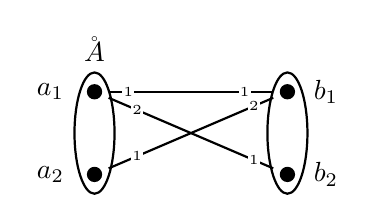
\begin{tikzpicture}[thick,  ncnode/.style={draw=black,,circle,fill=black,scale=0.5},  cnode/.style={draw=red,circle,fill=red,scale=0.5},
  every fit/.style={ellipse,draw,inner sep=-2pt,text width=0.5cm},  -,shorten >= 3pt,shorten <= 3pt, scale=0.7]

% the vertices of A U B
  \node[ncnode] (a1) at (-1,3) {};
  \node[ncnode] (a2) at (-1,1.5) {};
  \node[ncnode] (b1) at (2.5,3) {};
  \node[ncnode] (b2) at (2.5,1.5) {};
    \node at (-1.8,3) {$a_1$};
    \node at (-1.8,1.5) {$a_2$};
    \node at (3.2,3) {$b_1$};
    \node at (3.2,1.5) {$b_2$};


% the set A
\node [fit=(a1) (a2),label=above:$\AA$] {};
% the set B
\node [fit=(b1) (b2),label=above:$\BB$] {};

% the edges
\draw(a1) -- (b1) node[pos=0.15,draw=white, fill=white,inner sep=0.1pt] {\textcolor{black}{\tiny 1}} node[pos=0.8,draw=white, fill=white,inner sep=0.1pt] {\textcolor{black}{\tiny 1}};
\draw(a1) -- (b2) node[pos=0.2,draw=white,fill=white,inner sep=0.1pt]{\textcolor{black}{\tiny 2}} node[pos=0.85,draw=white, fill=white,inner sep=0.1pt] {\textcolor{black}{\tiny 1}};
\draw(a2) -- (b1) node[pos=0.2,draw=white,fill=white,inner sep=0.1pt]{\textcolor{black}{\tiny 1}} node[pos=0.85,draw=white, fill=white,inner sep=0.1pt] {\textcolor{black}{\tiny 2}};
\end{tikzpicture}

\caption{}
\label{subfig:popNOTrsm}
\end{subfigure}%
\begin{subfigure}{.5\textwidth}
\centering
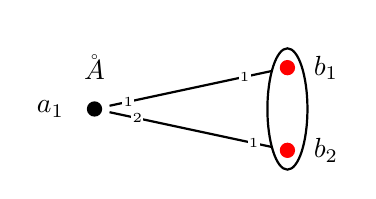
\begin{tikzpicture}[thick,  ncnode/.style={draw=black,,circle,fill=black,scale=0.5},  cnode/.style={draw=red,circle,fill=red,scale=0.5},
  every fit/.style={ellipse,draw,inner sep=-2pt,text width=0.5cm},  -,shorten >= 3pt,shorten <= 3pt, scale=0.7]

% the vertices of A U B
  \node[ncnode] (a1) at (-1,2.25) {};
  \node[cnode] (b1) at (2.5,3) {};
  \node[cnode] (b2) at (2.5,1.5) {};
    \node at (-1.8,2.25) {$a_1$};
    \node at (3.2,3) {$b_1$};
    \node at (3.2,1.5) {$b_2$};


% the set A
% \node [fit=(a1),label=above:$\AA$] {};
\node at (-1,3) {$\AA$};
% the set B
\node [fit=(b1) (b2),label=above:$\BB$] {};

% the edges
\draw(a1) -- (b1) node[pos=0.15,draw=white, fill=white,inner sep=0.1pt] {\textcolor{black}{\tiny 1}} node[pos=0.8,draw=white, fill=white,inner sep=0.1pt] {\textcolor{black}{\tiny 1}};
\draw(a1) -- (b2) node[pos=0.2,draw=white,fill=white,inner sep=0.1pt]{\textcolor{black}{\tiny 2}} node[pos=0.85,draw=white, fill=white,inner sep=0.1pt] {\textcolor{black}{\tiny 1}};
\end{tikzpicture}

\caption{}
\label{subfig:rsmNOTpop}
\end{subfigure}%
\caption{\label{fig:rsmNOTpop}%
The red vertices are critical and black vertices are non-critical. The numbers on the edges denote the ranking of the other endpoint in the preference list of that vertex.}
\end{figure}

	%
\end{document}
